\documentclass[11pt, a4paper]{report}

%%%%%%%%%%%%%%%%%%%%%%%%%%%%%%%%%
% PACKAGE IMPORTS
%%%%%%%%%%%%%%%%%%%%%%%%%%%%%%%%%


\usepackage[tmargin=2cm,rmargin=1in,lmargin=1in,margin=0.85in,bmargin=2cm,footskip=.2in]{geometry}
\usepackage{amsmath,amsfonts,amsthm,amssymb,mathtools}
\usepackage[varbb]{newpxmath}
\usepackage{xfrac}
\usepackage[makeroom]{cancel}
\usepackage{mathtools}
\usepackage{bookmark}
\usepackage{enumitem}
\usepackage{subcaption}
% \usepackage{physics}
\usepackage{hyperref,theoremref}
\hypersetup{
	pdftitle={Assignment},
	colorlinks=true, linkcolor=doc!90,
	bookmarksnumbered=true,
	bookmarksopen=true
}
\usepackage[most,many,breakable]{tcolorbox}
\usepackage{xcolor}
\usepackage{varwidth}
\usepackage{varwidth}
\usepackage{etoolbox}
%\usepackage{authblk}
\usepackage{nameref}
\usepackage{multicol,array}
\usepackage{tikz-cd}
\usepackage[ruled,vlined,linesnumbered]{algorithm2e}
\usepackage{comment} % enables the use of multi-line comments (\ifx \fi) 
\usepackage{import}
\usepackage{xifthen}
\usepackage{pdfpages}
\usepackage{transparent}

\newcommand\mycommfont[1]{\footnotesize\ttfamily\textcolor{blue}{#1}}
\SetCommentSty{mycommfont}
\newcommand{\incfig}[1]{%
    \def\svgwidth{\columnwidth}
    \import{./figures/}{#1.pdf_tex}
}

\usepackage{tikzsymbols}
\renewcommand\qedsymbol{$\Laughey$}


%\usepackage{import}
%\usepackage{xifthen}
%\usepackage{pdfpages}
%\usepackage{transparent}


%%%%%%%%%%%%%%%%%%%%%%%%%%%%%%
% SELF MADE COLORS
%%%%%%%%%%%%%%%%%%%%%%%%%%%%%%



\definecolor{myg}{RGB}{56, 140, 70}
\definecolor{myb}{RGB}{45, 111, 177}
\definecolor{myr}{RGB}{199, 68, 64}
\definecolor{mytheorembg}{HTML}{F2F2F9}
\definecolor{mytheoremfr}{HTML}{00007B}
\definecolor{mylenmabg}{HTML}{FFFAF8}
\definecolor{mylenmafr}{HTML}{983b0f}
\definecolor{mypropbg}{HTML}{f2fbfc}
\definecolor{mypropfr}{HTML}{191971}
\definecolor{myexamplebg}{HTML}{F2FBF8}
\definecolor{myexamplefr}{HTML}{88D6D1}
\definecolor{myexampleti}{HTML}{2A7F7F}
\definecolor{mydefinitbg}{HTML}{E5E5FF}
\definecolor{mydefinitfr}{HTML}{3F3FA3}
\definecolor{notesgreen}{RGB}{0,162,0}
\definecolor{myp}{RGB}{197, 92, 212}
\definecolor{mygr}{HTML}{2C3338}
\definecolor{myred}{RGB}{127,0,0}
\definecolor{myyellow}{RGB}{169,121,69}
\definecolor{myexercisebg}{HTML}{F2FBF8}
\definecolor{myexercisefg}{HTML}{88D6D1}


%%%%%%%%%%%%%%%%%%%%%%%%%%%%
% TCOLORBOX SETUPS
%%%%%%%%%%%%%%%%%%%%%%%%%%%%

\setlength{\parindent}{1cm}
%================================
% THEOREM BOX
%================================

\tcbuselibrary{theorems,skins,hooks}
\newtcbtheorem[number within=section]{Theorem}{Theorem}
{%
	enhanced,
	breakable,
	colback = mytheorembg,
	frame hidden,
	boxrule = 0sp,
	borderline west = {2pt}{0pt}{mytheoremfr},
	sharp corners,
	detach title,
	before upper = \tcbtitle\par\smallskip,
	coltitle = mytheoremfr,
	fonttitle = \bfseries\sffamily,
	description font = \mdseries,
	separator sign none,
	segmentation style={solid, mytheoremfr},
}
{th}

\tcbuselibrary{theorems,skins,hooks}
\newtcbtheorem[number within=chapter]{theorem}{Theorem}
{%
	enhanced,
	breakable,
	colback = mytheorembg,
	frame hidden,
	boxrule = 0sp,
	borderline west = {2pt}{0pt}{mytheoremfr},
	sharp corners,
	detach title,
	before upper = \tcbtitle\par\smallskip,
	coltitle = mytheoremfr,
	fonttitle = \bfseries\sffamily,
	description font = \mdseries,
	separator sign none,
	segmentation style={solid, mytheoremfr},
}
{th}


\tcbuselibrary{theorems,skins,hooks}
\newtcolorbox{Theoremcon}
{%
	enhanced
	,breakable
	,colback = mytheorembg
	,frame hidden
	,boxrule = 0sp
	,borderline west = {2pt}{0pt}{mytheoremfr}
	,sharp corners
	,description font = \mdseries
	,separator sign none
}

%================================
% Corollery
%================================
\tcbuselibrary{theorems,skins,hooks}
\newtcbtheorem[number within=section]{Corollary}{Corollary}
{%
	enhanced
	,breakable
	,colback = myp!10
	,frame hidden
	,boxrule = 0sp
	,borderline west = {2pt}{0pt}{myp!85!black}
	,sharp corners
	,detach title
	,before upper = \tcbtitle\par\smallskip
	,coltitle = myp!85!black
	,fonttitle = \bfseries\sffamily
	,description font = \mdseries
	,separator sign none
	,segmentation style={solid, myp!85!black}
}
{th}
\tcbuselibrary{theorems,skins,hooks}
\newtcbtheorem[number within=chapter]{corollary}{Corollary}
{%
	enhanced
	,breakable
	,colback = myp!10
	,frame hidden
	,boxrule = 0sp
	,borderline west = {2pt}{0pt}{myp!85!black}
	,sharp corners
	,detach title
	,before upper = \tcbtitle\par\smallskip
	,coltitle = myp!85!black
	,fonttitle = \bfseries\sffamily
	,description font = \mdseries
	,separator sign none
	,segmentation style={solid, myp!85!black}
}
{th}


%================================
% LENMA
%================================

\tcbuselibrary{theorems,skins,hooks}
\newtcbtheorem[number within=section]{Lenma}{Lenma}
{%
	enhanced,
	breakable,
	colback = mylenmabg,
	frame hidden,
	boxrule = 0sp,
	borderline west = {2pt}{0pt}{mylenmafr},
	sharp corners,
	detach title,
	before upper = \tcbtitle\par\smallskip,
	coltitle = mylenmafr,
	fonttitle = \bfseries\sffamily,
	description font = \mdseries,
	separator sign none,
	segmentation style={solid, mylenmafr},
}
{th}

\tcbuselibrary{theorems,skins,hooks}
\newtcbtheorem[number within=chapter]{lenma}{Lenma}
{%
	enhanced,
	breakable,
	colback = mylenmabg,
	frame hidden,
	boxrule = 0sp,
	borderline west = {2pt}{0pt}{mylenmafr},
	sharp corners,
	detach title,
	before upper = \tcbtitle\par\smallskip,
	coltitle = mylenmafr,
	fonttitle = \bfseries\sffamily,
	description font = \mdseries,
	separator sign none,
	segmentation style={solid, mylenmafr},
}
{th}


%================================
% PROPOSITION
%================================

\tcbuselibrary{theorems,skins,hooks}
\newtcbtheorem[number within=section]{Prop}{Proposition}
{%
	enhanced,
	breakable,
	colback = mypropbg,
	frame hidden,
	boxrule = 0sp,
	borderline west = {2pt}{0pt}{mypropfr},
	sharp corners,
	detach title,
	before upper = \tcbtitle\par\smallskip,
	coltitle = mypropfr,
	fonttitle = \bfseries\sffamily,
	description font = \mdseries,
	separator sign none,
	segmentation style={solid, mypropfr},
}
{th}

\tcbuselibrary{theorems,skins,hooks}
\newtcbtheorem[number within=chapter]{prop}{Proposition}
{%
	enhanced,
	breakable,
	colback = mypropbg,
	frame hidden,
	boxrule = 0sp,
	borderline west = {2pt}{0pt}{mypropfr},
	sharp corners,
	detach title,
	before upper = \tcbtitle\par\smallskip,
	coltitle = mypropfr,
	fonttitle = \bfseries\sffamily,
	description font = \mdseries,
	separator sign none,
	segmentation style={solid, mypropfr},
}
{th}


%================================
% CLAIM
%================================

\tcbuselibrary{theorems,skins,hooks}
\newtcbtheorem[number within=section]{claim}{Claim}
{%
	enhanced
	,breakable
	,colback = myg!10
	,frame hidden
	,boxrule = 0sp
	,borderline west = {2pt}{0pt}{myg}
	,sharp corners
	,detach title
	,before upper = \tcbtitle\par\smallskip
	,coltitle = myg!85!black
	,fonttitle = \bfseries\sffamily
	,description font = \mdseries
	,separator sign none
	,segmentation style={solid, myg!85!black}
}
{th}



%================================
% Exercise
%================================

\tcbuselibrary{theorems,skins,hooks}
\newtcbtheorem[number within=section]{Exercise}{Exercise}
{%
	enhanced,
	breakable,
	colback = myexercisebg,
	frame hidden,
	boxrule = 0sp,
	borderline west = {2pt}{0pt}{myexercisefg},
	sharp corners,
	detach title,
	before upper = \tcbtitle\par\smallskip,
	coltitle = myexercisefg,
	fonttitle = \bfseries\sffamily,
	description font = \mdseries,
	separator sign none,
	segmentation style={solid, myexercisefg},
}
{th}

\tcbuselibrary{theorems,skins,hooks}
\newtcbtheorem[number within=chapter]{exercise}{Exercise}
{%
	enhanced,
	breakable,
	colback = myexercisebg,
	frame hidden,
	boxrule = 0sp,
	borderline west = {2pt}{0pt}{myexercisefg},
	sharp corners,
	detach title,
	before upper = \tcbtitle\par\smallskip,
	coltitle = myexercisefg,
	fonttitle = \bfseries\sffamily,
	description font = \mdseries,
	separator sign none,
	segmentation style={solid, myexercisefg},
}
{th}

%================================
% EXAMPLE BOX
%================================

\newtcbtheorem[number within=section]{Example}{Example}
{%
	colback = myexamplebg
	,breakable
	,colframe = myexamplefr
	,coltitle = myexampleti
	,boxrule = 1pt
	,sharp corners
	,detach title
	,before upper=\tcbtitle\par\smallskip
	,fonttitle = \bfseries
	,description font = \mdseries
	,separator sign none
	,description delimiters parenthesis
}
{ex}

\newtcbtheorem[number within=chapter]{example}{Example}
{%
	colback = myexamplebg
	,breakable
	,colframe = myexamplefr
	,coltitle = myexampleti
	,boxrule = 1pt
	,sharp corners
	,detach title
	,before upper=\tcbtitle\par\smallskip
	,fonttitle = \bfseries
	,description font = \mdseries
	,separator sign none
	,description delimiters parenthesis
}
{ex}

%================================
% DEFINITION BOX
%================================

\newtcbtheorem[number within=section]{Definition}{Definition}{enhanced,
	before skip=2mm,after skip=2mm, colback=red!5,colframe=red!80!black,boxrule=0.5mm,
	attach boxed title to top left={xshift=1cm,yshift*=1mm-\tcboxedtitleheight}, varwidth boxed title*=-3cm,
	boxed title style={frame code={
					\path[fill=tcbcolback]
					([yshift=-1mm,xshift=-1mm]frame.north west)
					arc[start angle=0,end angle=180,radius=1mm]
					([yshift=-1mm,xshift=1mm]frame.north east)
					arc[start angle=180,end angle=0,radius=1mm];
					\path[left color=tcbcolback!60!black,right color=tcbcolback!60!black,
						middle color=tcbcolback!80!black]
					([xshift=-2mm]frame.north west) -- ([xshift=2mm]frame.north east)
					[rounded corners=1mm]-- ([xshift=1mm,yshift=-1mm]frame.north east)
					-- (frame.south east) -- (frame.south west)
					-- ([xshift=-1mm,yshift=-1mm]frame.north west)
					[sharp corners]-- cycle;
				},interior engine=empty,
		},
	fonttitle=\bfseries,
	title={#2},#1}{def}
\newtcbtheorem[number within=chapter]{definition}{Definition}{enhanced,
	before skip=2mm,after skip=2mm, colback=red!5,colframe=red!80!black,boxrule=0.5mm,
	attach boxed title to top left={xshift=1cm,yshift*=1mm-\tcboxedtitleheight}, varwidth boxed title*=-3cm,
	boxed title style={frame code={
					\path[fill=tcbcolback]
					([yshift=-1mm,xshift=-1mm]frame.north west)
					arc[start angle=0,end angle=180,radius=1mm]
					([yshift=-1mm,xshift=1mm]frame.north east)
					arc[start angle=180,end angle=0,radius=1mm];
					\path[left color=tcbcolback!60!black,right color=tcbcolback!60!black,
						middle color=tcbcolback!80!black]
					([xshift=-2mm]frame.north west) -- ([xshift=2mm]frame.north east)
					[rounded corners=1mm]-- ([xshift=1mm,yshift=-1mm]frame.north east)
					-- (frame.south east) -- (frame.south west)
					-- ([xshift=-1mm,yshift=-1mm]frame.north west)
					[sharp corners]-- cycle;
				},interior engine=empty,
		},
	fonttitle=\bfseries,
	title={#2},#1}{def}



%================================
% Solution BOX
%================================

\makeatletter
\newtcbtheorem{question}{Question}{enhanced,
	breakable,
	colback=white,
	colframe=myb!80!black,
	attach boxed title to top left={yshift*=-\tcboxedtitleheight},
	fonttitle=\bfseries,
	title={#2},
	boxed title size=title,
	boxed title style={%
			sharp corners,
			rounded corners=northwest,
			colback=tcbcolframe,
			boxrule=0pt,
		},
	underlay boxed title={%
			\path[fill=tcbcolframe] (title.south west)--(title.south east)
			to[out=0, in=180] ([xshift=5mm]title.east)--
			(title.center-|frame.east)
			[rounded corners=\kvtcb@arc] |-
			(frame.north) -| cycle;
		},
	#1
}{def}
\makeatother

%================================
% SOLUTION BOX
%================================

\makeatletter
\newtcolorbox{solution}{enhanced,
	breakable,
	colback=white,
	colframe=myg!80!black,
	attach boxed title to top left={yshift*=-\tcboxedtitleheight},
	title=Solution,
	boxed title size=title,
	boxed title style={%
			sharp corners,
			rounded corners=northwest,
			colback=tcbcolframe,
			boxrule=0pt,
		},
	underlay boxed title={%
			\path[fill=tcbcolframe] (title.south west)--(title.south east)
			to[out=0, in=180] ([xshift=5mm]title.east)--
			(title.center-|frame.east)
			[rounded corners=\kvtcb@arc] |-
			(frame.north) -| cycle;
		},
}
\makeatother

%================================
% Question BOX
%================================

\makeatletter
\newtcbtheorem{qstion}{Question}{enhanced,
	breakable,
	colback=white,
	colframe=mygr,
	attach boxed title to top left={yshift*=-\tcboxedtitleheight},
	fonttitle=\bfseries,
	title={#2},
	boxed title size=title,
	boxed title style={%
			sharp corners,
			rounded corners=northwest,
			colback=tcbcolframe,
			boxrule=0pt,
		},
	underlay boxed title={%
			\path[fill=tcbcolframe] (title.south west)--(title.south east)
			to[out=0, in=180] ([xshift=5mm]title.east)--
			(title.center-|frame.east)
			[rounded corners=\kvtcb@arc] |-
			(frame.north) -| cycle;
		},
	#1
}{def}
\makeatother

\newtcbtheorem[number within=chapter]{wconc}{Wrong Concept}{
	breakable,
	enhanced,
	colback=white,
	colframe=myr,
	arc=0pt,
	outer arc=0pt,
	fonttitle=\bfseries\sffamily\large,
	colbacktitle=myr,
	attach boxed title to top left={},
	boxed title style={
			enhanced,
			skin=enhancedfirst jigsaw,
			arc=3pt,
			bottom=0pt,
			interior style={fill=myr}
		},
	#1
}{def}



%================================
% NOTE BOX
%================================

\usetikzlibrary{arrows,calc,shadows.blur}
\tcbuselibrary{skins}
\newtcolorbox{note}[1][]{%
	enhanced jigsaw,
	colback=gray!20!white,%
	colframe=gray!80!black,
	size=small,
	boxrule=1pt,
	title=\textbf{Note:-},
	halign title=flush center,
	coltitle=black,
	breakable,
	drop shadow=black!50!white,
	attach boxed title to top left={xshift=1cm,yshift=-\tcboxedtitleheight/2,yshifttext=-\tcboxedtitleheight/2},
	minipage boxed title=1.5cm,
	boxed title style={%
			colback=white,
			size=fbox,
			boxrule=1pt,
			boxsep=2pt,
			underlay={%
					\coordinate (dotA) at ($(interior.west) + (-0.5pt,0)$);
					\coordinate (dotB) at ($(interior.east) + (0.5pt,0)$);
					\begin{scope}
						\clip (interior.north west) rectangle ([xshift=3ex]interior.east);
						\filldraw [white, blur shadow={shadow opacity=60, shadow yshift=-.75ex}, rounded corners=2pt] (interior.north west) rectangle (interior.south east);
					\end{scope}
					\begin{scope}[gray!80!black]
						\fill (dotA) circle (2pt);
						\fill (dotB) circle (2pt);
					\end{scope}
				},
		},
	#1,
}

%%%%%%%%%%%%%%%%%%%%%%%%%%%%%%
% SELF MADE COMMANDS
%%%%%%%%%%%%%%%%%%%%%%%%%%%%%%


\newcommand{\thm}[2]{\begin{Theorem}{#1}{}#2\end{Theorem}}
\newcommand{\cor}[2]{\begin{Corollary}{#1}{}#2\end{Corollary}}
\newcommand{\mlenma}[2]{\begin{Lenma}{#1}{}#2\end{Lenma}}
\newcommand{\mprop}[2]{\begin{Prop}{#1}{}#2\end{Prop}}
\newcommand{\clm}[3]{\begin{claim}{#1}{#2}#3\end{claim}}
\newcommand{\wc}[2]{\begin{wconc}{#1}{}\setlength{\parindent}{1cm}#2\end{wconc}}
\newcommand{\thmcon}[1]{\begin{Theoremcon}{#1}\end{Theoremcon}}
\newcommand{\ex}[2]{\begin{Example}{#1}{}#2\end{Example}}
\newcommand{\dfn}[2]{\begin{Definition}[colbacktitle=red!75!black]{#1}{}#2\end{Definition}}
\newcommand{\dfnc}[2]{\begin{definition}[colbacktitle=red!75!black]{#1}{}#2\end{definition}}
\newcommand{\qs}[2]{\begin{question}{#1}{}#2\end{question}}
\newcommand{\pf}[2]{\begin{myproof}[#1]#2\end{myproof}}
\newcommand{\nt}[1]{\begin{note}#1\end{note}}

\newcommand*\circled[1]{\tikz[baseline=(char.base)]{
		\node[shape=circle,draw,inner sep=1pt] (char) {#1};}}
\newcommand\getcurrentref[1]{%
	\ifnumequal{\value{#1}}{0}
	{??}
	{\the\value{#1}}%
}
\newcommand{\getCurrentSectionNumber}{\getcurrentref{section}}
\newenvironment{myproof}[1][\proofname]{%
	\proof[\bfseries #1: ]%
}{\endproof}

\newcommand{\mclm}[2]{\begin{myclaim}[#1]#2\end{myclaim}}
\newenvironment{myclaim}[1][\claimname]{\proof[\bfseries #1: ]}{}

\newcounter{mylabelcounter}

\makeatletter
\newcommand{\setword}[2]{%
	\phantomsection
	#1\def\@currentlabel{\unexpanded{#1}}\label{#2}%
}
\makeatother




\tikzset{
	symbol/.style={
			draw=none,
			every to/.append style={
					edge node={node [sloped, allow upside down, auto=false]{$#1$}}}
		}
}


% deliminators
\DeclarePairedDelimiter{\abs}{\lvert}{\rvert}
\DeclarePairedDelimiter{\norm}{\lVert}{\rVert}

\DeclarePairedDelimiter{\ceil}{\lceil}{\rceil}
\DeclarePairedDelimiter{\floor}{\lfloor}{\rfloor}
\DeclarePairedDelimiter{\round}{\lfloor}{\rceil}

\newsavebox\diffdbox
\newcommand{\slantedromand}{{\mathpalette\makesl{d}}}
\newcommand{\makesl}[2]{%
\begingroup
\sbox{\diffdbox}{$\mathsurround=0pt#1\mathrm{#2}$}%
\pdfsave
\pdfsetmatrix{1 0 0.2 1}%
\rlap{\usebox{\diffdbox}}%
\pdfrestore
\hskip\wd\diffdbox
\endgroup
}
\newcommand{\dd}[1][]{\ensuremath{\mathop{}\!\ifstrempty{#1}{%
\slantedromand\@ifnextchar^{\hspace{0.2ex}}{\hspace{0.1ex}}}%
{\slantedromand\hspace{0.2ex}^{#1}}}}
\ProvideDocumentCommand\dv{o m g}{%
  \ensuremath{%
    \IfValueTF{#3}{%
      \IfNoValueTF{#1}{%
        \frac{\dd #2}{\dd #3}%
      }{%
        \frac{\dd^{#1} #2}{\dd #3^{#1}}%
      }%
    }{%
      \IfNoValueTF{#1}{%
        \frac{\dd}{\dd #2}%
      }{%
        \frac{\dd^{#1}}{\dd #2^{#1}}%
      }%
    }%
  }%
}
\providecommand*{\pdv}[3][]{\frac{\partial^{#1}#2}{\partial#3^{#1}}}
%  - others
\DeclareMathOperator{\Lap}{\mathcal{L}}
\DeclareMathOperator{\Var}{Var} % varience
\DeclareMathOperator{\Cov}{Cov} % covarience
\DeclareMathOperator{\E}{E} % expected

% Since the amsthm package isn't loaded

% I prefer the slanted \leq
\let\oldleq\leq % save them in case they're every wanted
\let\oldgeq\geq
\renewcommand{\leq}{\leqslant}
\renewcommand{\geq}{\geqslant}

% % redefine matrix env to allow for alignment, use r as default
% \renewcommand*\env@matrix[1][r]{\hskip -\arraycolsep
%     \let\@ifnextchar\new@ifnextchar
%     \array{*\c@MaxMatrixCols #1}}


%\usepackage{framed}
%\usepackage{titletoc}
%\usepackage{etoolbox}
%\usepackage{lmodern}


%\patchcmd{\tableofcontents}{\contentsname}{\sffamily\contentsname}{}{}

%\renewenvironment{leftbar}
%{\def\FrameCommand{\hspace{6em}%
%		{\color{myyellow}\vrule width 2pt depth 6pt}\hspace{1em}}%
%	\MakeFramed{\parshape 1 0cm \dimexpr\textwidth-6em\relax\FrameRestore}\vskip2pt%
%}
%{\endMakeFramed}

%\titlecontents{chapter}
%[0em]{\vspace*{2\baselineskip}}
%{\parbox{4.5em}{%
%		\hfill\Huge\sffamily\bfseries\color{myred}\thecontentspage}%
%	\vspace*{-2.3\baselineskip}\leftbar\textsc{\small\chaptername~\thecontentslabel}\\\sffamily}
%{}{\endleftbar}
%\titlecontents{section}
%[8.4em]
%{\sffamily\contentslabel{3em}}{}{}
%{\hspace{0.5em}\nobreak\itshape\color{myred}\contentspage}
%\titlecontents{subsection}
%[8.4em]
%{\sffamily\contentslabel{3em}}{}{}  
%{\hspace{0.5em}\nobreak\itshape\color{myred}\contentspage}



%%%%%%%%%%%%%%%%%%%%%%%%%%%%%%%%%%%%%%%%%%%
% TABLE OF CONTENTS
%%%%%%%%%%%%%%%%%%%%%%%%%%%%%%%%%%%%%%%%%%%

\usepackage{tikz}
\definecolor{doc}{RGB}{0,60,110}
\usepackage{titletoc}
\contentsmargin{0cm}
\titlecontents{chapter}[3.7pc]
{\addvspace{30pt}%
	\begin{tikzpicture}[remember picture, overlay]%
		\draw[fill=doc!60,draw=doc!60] (-7,-.1) rectangle (-0.9,.5);%
		\pgftext[left,x=-3.5cm,y=0.2cm]{\color{white}\Large\sc\bfseries Chapter\ \thecontentslabel};%
	\end{tikzpicture}\color{doc!60}\large\sc\bfseries}%
{}
{}
{\;\titlerule\;\large\sc\bfseries Page \thecontentspage
	\begin{tikzpicture}[remember picture, overlay]
		\draw[fill=doc!60,draw=doc!60] (2pt,0) rectangle (4,0.1pt);
	\end{tikzpicture}}%
\titlecontents{section}[3.7pc]
{\addvspace{2pt}}
{\contentslabel[\thecontentslabel]{2pc}}
{}
{\hfill\small \thecontentspage}
[]
\titlecontents*{subsection}[3.7pc]
{\addvspace{-1pt}\small}
{}
{}
{\ --- \small\thecontentspage}
[ \textbullet\ ][]

\makeatletter
\renewcommand{\tableofcontents}{%
	\chapter*{%
	  \vspace*{-20\p@}%
	  \begin{tikzpicture}[remember picture, overlay]%
		  \pgftext[right,x=15cm,y=0.2cm]{\color{doc!60}\Huge\sc\bfseries \contentsname};%
		  \draw[fill=doc!60,draw=doc!60] (13,-.75) rectangle (20,1);%
		  \clip (13,-.75) rectangle (20,1);
		  \pgftext[right,x=15cm,y=0.2cm]{\color{white}\Huge\sc\bfseries \contentsname};%
	  \end{tikzpicture}}%
	\@starttoc{toc}}
\makeatother


\usepackage[svgnames]{xcolor} % Required to specify font color

\newcommand*{\plogo}{\fbox{$\mathcal{PL}$}} % Generic publisher logo

\usepackage{graphicx} % Required for box manipulation

%----------------------------------------------------------------------------------------
%	TITLE PAGE
%----------------------------------------------------------------------------------------

\newcommand*{\rotrt}[1]{\rotatebox{90}{#1}} % Command to rotate right 90 degrees
\newcommand*{\rotlft}[1]{\rotatebox{-90}{#1}} % Command to rotate left 90 degrees

\newcommand*{\titleBC}{\begingroup % Create the command for including the title page in the document
\centering % Center all text

\def\CP{\textit{\Huge Queueing Theory - Seminar Notes}} % Title

\settowidth{\unitlength}{\CP} % Set the width of the curly brackets to the width of the title
{\color{LightGoldenrod}\resizebox*{\unitlength}{\baselineskip}{\rotrt{$\}$}}} \\[\baselineskip] % Print top curly bracket
\textcolor{Sienna}{\CP} \\[\baselineskip] % Print title
{\color{RosyBrown}\Large A Mathematically-Rigorous yet Intuitive Introduction to Queues} \\ % Tagline or further description
{\color{LightGoldenrod}\resizebox*{\unitlength}{\baselineskip}{\rotlft{$\}$}}} % Print bottom curly bracket

\vfill % Whitespace between the title and the author name

{\Large\textbf{Rishabh Pomaje}\\ \href{mailto:210020036@iitdh.ac.in}{210020036@iitdh.ac.in}}\\ % Author name

\vfill % Whitespace between the author name and the publisher logo

\endgroup}

%From M275 "Topology" at SJSU
\newcommand{\id}{\mathrm{id}}
\newcommand{\taking}[1]{\xrightarrow{#1}}
\newcommand{\inv}{^{-1}}

%From M170 "Introduction to Graph Theory" at SJSU
\DeclareMathOperator{\diam}{diam}
\DeclareMathOperator{\ord}{ord}
\newcommand{\defeq}{\overset{\mathrm{def}}{=}}

%From the USAMO .tex files
\newcommand{\ts}{\textsuperscript}
\newcommand{\dg}{^\circ}
\newcommand{\ii}{\item}

% % From Math 55 and Math 145 at Harvard
% \newenvironment{subproof}[1][Proof]{%
% \begin{proof}[#1] \renewcommand{\qedsymbol}{$\blacksquare$}}%
% {\end{proof}}

\newcommand{\liff}{\leftrightarrow}
\newcommand{\lthen}{\rightarrow}
\newcommand{\opname}{\operatorname}
\newcommand{\surjto}{\twoheadrightarrow}
\newcommand{\injto}{\hookrightarrow}
\newcommand{\On}{\mathrm{On}} % ordinals
\DeclareMathOperator{\img}{im} % Image
\DeclareMathOperator{\Img}{Im} % Image
\DeclareMathOperator{\coker}{coker} % Cokernel
\DeclareMathOperator{\Coker}{Coker} % Cokernel
\DeclareMathOperator{\Ker}{Ker} % Kernel
\DeclareMathOperator{\rank}{rank}
\DeclareMathOperator{\Spec}{Spec} % spectrum
\DeclareMathOperator{\Tr}{Tr} % trace
\DeclareMathOperator{\pr}{pr} % projection
\DeclareMathOperator{\ext}{ext} % extension
\DeclareMathOperator{\pred}{pred} % predecessor
\DeclareMathOperator{\dom}{dom} % domain
\DeclareMathOperator{\ran}{ran} % range
\DeclareMathOperator{\Hom}{Hom} % homomorphism
\DeclareMathOperator{\Mor}{Mor} % morphisms
\DeclareMathOperator{\End}{End} % endomorphism

\newcommand{\eps}{\epsilon}
\newcommand{\veps}{\varepsilon}
\newcommand{\ol}{\overline}
\newcommand{\ul}{\underline}
\newcommand{\wt}{\widetilde}
\newcommand{\wh}{\widehat}
\newcommand{\vocab}[1]{\textbf{\color{blue} #1}}
\providecommand{\half}{\frac{1}{2}}
\newcommand{\dang}{\measuredangle} %% Directed angle
\newcommand{\ray}[1]{\overrightarrow{#1}}
\newcommand{\seg}[1]{\overline{#1}}
\newcommand{\arc}[1]{\wideparen{#1}}
\DeclareMathOperator{\cis}{cis}
\DeclareMathOperator*{\lcm}{lcm}
\DeclareMathOperator*{\argmin}{arg min}
\DeclareMathOperator*{\argmax}{arg max}
\newcommand{\cycsum}{\sum_{\mathrm{cyc}}}
\newcommand{\symsum}{\sum_{\mathrm{sym}}}
\newcommand{\cycprod}{\prod_{\mathrm{cyc}}}
\newcommand{\symprod}{\prod_{\mathrm{sym}}}
\newcommand{\Qed}{\begin{flushright}\qed\end{flushright}}
\newcommand{\parinn}{\setlength{\parindent}{1cm}}
\newcommand{\parinf}{\setlength{\parindent}{0cm}}
% \newcommand{\norm}{\|\cdot\|}
\newcommand{\inorm}{\norm_{\infty}}
\newcommand{\opensets}{\{V_{\alpha}\}_{\alpha\in I}}
\newcommand{\oset}{V_{\alpha}}
\newcommand{\opset}[1]{V_{\alpha_{#1}}}
\newcommand{\lub}{\text{lub}}
\newcommand{\del}[2]{\frac{\partial #1}{\partial #2}}
\newcommand{\Del}[3]{\frac{\partial^{#1} #2}{\partial^{#1} #3}}
\newcommand{\deld}[2]{\dfrac{\partial #1}{\partial #2}}
\newcommand{\Deld}[3]{\dfrac{\partial^{#1} #2}{\partial^{#1} #3}}
\newcommand{\lm}{\lambda}
\newcommand{\uin}{\mathbin{\rotatebox[origin=c]{90}{$\in$}}}
\newcommand{\usubset}{\mathbin{\rotatebox[origin=c]{90}{$\subset$}}}
\newcommand{\lt}{\left}
\newcommand{\rt}{\right}
\newcommand{\bs}[1]{\boldsymbol{#1}}
\newcommand{\exs}{\exists}
\newcommand{\st}{\strut}
\newcommand{\dps}[1]{\displaystyle{#1}}

\newcommand{\sol}{\setlength{\parindent}{0cm}\textbf{\textit{Solution:}}\setlength{\parindent}{1cm} }
\newcommand{\solve}[1]{\setlength{\parindent}{0cm}\textbf{\textit{Solution: }}\setlength{\parindent}{1cm}#1 \Qed}

%%%%% NEW MATH DEFINITIONS %%%%%

\usepackage{amsmath,amsfonts,bm}

% Mark sections of captions for referring to divisions of figures
\newcommand{\figleft}{{\em (Left)}}
\newcommand{\figcenter}{{\em (Center)}}
\newcommand{\figright}{{\em (Right)}}
\newcommand{\figtop}{{\em (Top)}}
\newcommand{\figbottom}{{\em (Bottom)}}
\newcommand{\captiona}{{\em (a)}}
\newcommand{\captionb}{{\em (b)}}
\newcommand{\captionc}{{\em (c)}}
\newcommand{\captiond}{{\em (d)}}

% Highlight a newly defined term
\newcommand{\newterm}[1]{{\bf #1}}


% Figure reference, lower-case.
\def\figref#1{figure~\ref{#1}}
% Figure reference, capital. For start of sentence
\def\Figref#1{Figure~\ref{#1}}
\def\twofigref#1#2{figures \ref{#1} and \ref{#2}}
\def\quadfigref#1#2#3#4{figures \ref{#1}, \ref{#2}, \ref{#3} and \ref{#4}}
% Section reference, lower-case.
\def\secref#1{section~\ref{#1}}
% Section reference, capital.
\def\Secref#1{Section~\ref{#1}}
% Reference to two sections.
\def\twosecrefs#1#2{sections \ref{#1} and \ref{#2}}
% Reference to three sections.
\def\secrefs#1#2#3{sections \ref{#1}, \ref{#2} and \ref{#3}}
% Reference to an equation, lower-case.
\def\eqref#1{equation~\ref{#1}}
% Reference to an equation, upper case
\def\Eqref#1{Equation~\ref{#1}}
% A raw reference to an equation---avoid using if possible
\def\plaineqref#1{\ref{#1}}
% Reference to a chapter, lower-case.
\def\chapref#1{chapter~\ref{#1}}
% Reference to an equation, upper case.
\def\Chapref#1{Chapter~\ref{#1}}
% Reference to a range of chapters
\def\rangechapref#1#2{chapters\ref{#1}--\ref{#2}}
% Reference to an algorithm, lower-case.
\def\algref#1{algorithm~\ref{#1}}
% Reference to an algorithm, upper case.
\def\Algref#1{Algorithm~\ref{#1}}
\def\twoalgref#1#2{algorithms \ref{#1} and \ref{#2}}
\def\Twoalgref#1#2{Algorithms \ref{#1} and \ref{#2}}
% Reference to a part, lower case
\def\partref#1{part~\ref{#1}}
% Reference to a part, upper case
\def\Partref#1{Part~\ref{#1}}
\def\twopartref#1#2{parts \ref{#1} and \ref{#2}}

\def\ceil#1{\lceil #1 \rceil}
\def\floor#1{\lfloor #1 \rfloor}
\def\1{\bm{1}}
\newcommand{\train}{\mathcal{D}}
\newcommand{\valid}{\mathcal{D_{\mathrm{valid}}}}
\newcommand{\test}{\mathcal{D_{\mathrm{test}}}}

\def\eps{{\epsilon}}


% Random variables
% My definition
\def\ExpVal{{\mathbb{E}}}
%
\def\reta{{\textnormal{$\eta$}}}
\def\ra{{\textnormal{a}}}
\def\rb{{\textnormal{b}}}
\def\rc{{\textnormal{c}}}
\def\rd{{\textnormal{d}}}
\def\re{{\textnormal{e}}}
\def\rf{{\textnormal{f}}}
\def\rg{{\textnormal{g}}}
\def\rh{{\textnormal{h}}}
\def\ri{{\textnormal{i}}}
\def\rj{{\textnormal{j}}}
\def\rk{{\textnormal{k}}}
\def\rl{{\textnormal{l}}}
% rm is already a command, just don't name any random variables m
\def\rn{{\textnormal{n}}}
\def\ro{{\textnormal{o}}}
\def\rp{{\textnormal{p}}}
\def\rq{{\textnormal{q}}}
\def\rr{{\textnormal{r}}}
\def\rs{{\textnormal{s}}}
\def\rt{{\textnormal{t}}}
\def\ru{{\textnormal{u}}}
\def\rv{{\textnormal{v}}}
\def\rw{{\textnormal{w}}}
\def\rx{{\textnormal{x}}}
\def\ry{{\textnormal{y}}}
\def\rz{{\textnormal{z}}}

% Random vectors
\def\rvepsilon{{\mathbf{\epsilon}}}
\def\rvtheta{{\mathbf{\theta}}}
\def\rva{{\mathbf{a}}}
\def\rvb{{\mathbf{b}}}
\def\rvc{{\mathbf{c}}}
\def\rvd{{\mathbf{d}}}
\def\rve{{\mathbf{e}}}
\def\rvf{{\mathbf{f}}}
\def\rvg{{\mathbf{g}}}
\def\rvh{{\mathbf{h}}}
\def\rvu{{\mathbf{i}}}
\def\rvj{{\mathbf{j}}}
\def\rvk{{\mathbf{k}}}
\def\rvl{{\mathbf{l}}}
\def\rvm{{\mathbf{m}}}
\def\rvn{{\mathbf{n}}}
\def\rvo{{\mathbf{o}}}
\def\rvp{{\mathbf{p}}}
\def\rvq{{\mathbf{q}}}
\def\rvr{{\mathbf{r}}}
\def\rvs{{\mathbf{s}}}
\def\rvt{{\mathbf{t}}}
\def\rvu{{\mathbf{u}}}
\def\rvv{{\mathbf{v}}}
\def\rvw{{\mathbf{w}}}
\def\rvx{{\mathbf{x}}}
\def\rvy{{\mathbf{y}}}
\def\rvz{{\mathbf{z}}}

% Elements of random vectors
\def\erva{{\textnormal{a}}}
\def\ervb{{\textnormal{b}}}
\def\ervc{{\textnormal{c}}}
\def\ervd{{\textnormal{d}}}
\def\erve{{\textnormal{e}}}
\def\ervf{{\textnormal{f}}}
\def\ervg{{\textnormal{g}}}
\def\ervh{{\textnormal{h}}}
\def\ervi{{\textnormal{i}}}
\def\ervj{{\textnormal{j}}}
\def\ervk{{\textnormal{k}}}
\def\ervl{{\textnormal{l}}}
\def\ervm{{\textnormal{m}}}
\def\ervn{{\textnormal{n}}}
\def\ervo{{\textnormal{o}}}
\def\ervp{{\textnormal{p}}}
\def\ervq{{\textnormal{q}}}
\def\ervr{{\textnormal{r}}}
\def\ervs{{\textnormal{s}}}
\def\ervt{{\textnormal{t}}}
\def\ervu{{\textnormal{u}}}
\def\ervv{{\textnormal{v}}}
\def\ervw{{\textnormal{w}}}
\def\ervx{{\textnormal{x}}}
\def\ervy{{\textnormal{y}}}
\def\ervz{{\textnormal{z}}}

% Random matrices
\def\rmA{{\mathbf{A}}}
\def\rmB{{\mathbf{B}}}
\def\rmC{{\mathbf{C}}}
\def\rmD{{\mathbf{D}}}
\def\rmE{{\mathbf{E}}}
\def\rmF{{\mathbf{F}}}
\def\rmG{{\mathbf{G}}}
\def\rmH{{\mathbf{H}}}
\def\rmI{{\mathbf{I}}}
\def\rmJ{{\mathbf{J}}}
\def\rmK{{\mathbf{K}}}
\def\rmL{{\mathbf{L}}}
\def\rmM{{\mathbf{M}}}
\def\rmN{{\mathbf{N}}}
\def\rmO{{\mathbf{O}}}
\def\rmP{{\mathbf{P}}}
\def\rmQ{{\mathbf{Q}}}
\def\rmR{{\mathbf{R}}}
\def\rmS{{\mathbf{S}}}
\def\rmT{{\mathbf{T}}}
\def\rmU{{\mathbf{U}}}
\def\rmV{{\mathbf{V}}}
\def\rmW{{\mathbf{W}}}
\def\rmX{{\mathbf{X}}}
\def\rmY{{\mathbf{Y}}}
\def\rmZ{{\mathbf{Z}}}

% Elements of random matrices
\def\ermA{{\textnormal{A}}}
\def\ermB{{\textnormal{B}}}
\def\ermC{{\textnormal{C}}}
\def\ermD{{\textnormal{D}}}
\def\ermE{{\textnormal{E}}}
\def\ermF{{\textnormal{F}}}
\def\ermG{{\textnormal{G}}}
\def\ermH{{\textnormal{H}}}
\def\ermI{{\textnormal{I}}}
\def\ermJ{{\textnormal{J}}}
\def\ermK{{\textnormal{K}}}
\def\ermL{{\textnormal{L}}}
\def\ermM{{\textnormal{M}}}
\def\ermN{{\textnormal{N}}}
\def\ermO{{\textnormal{O}}}
\def\ermP{{\textnormal{P}}}
\def\ermQ{{\textnormal{Q}}}
\def\ermR{{\textnormal{R}}}
\def\ermS{{\textnormal{S}}}
\def\ermT{{\textnormal{T}}}
\def\ermU{{\textnormal{U}}}
\def\ermV{{\textnormal{V}}}
\def\ermW{{\textnormal{W}}}
\def\ermX{{\textnormal{X}}}
\def\ermY{{\textnormal{Y}}}
\def\ermZ{{\textnormal{Z}}}

% Vectors
\def\vzero{{\bm{0}}}
\def\vone{{\bm{1}}}
\def\vmu{{\bm{\mu}}}
\def\vtheta{{\bm{\theta}}}
\def\va{{\bm{a}}}
\def\vb{{\bm{b}}}
\def\vc{{\bm{c}}}
\def\vd{{\bm{d}}}
\def\ve{{\bm{e}}}
\def\vf{{\bm{f}}}
\def\vg{{\bm{g}}}
\def\vh{{\bm{h}}}
\def\vi{{\bm{i}}}
\def\vj{{\bm{j}}}
\def\vk{{\bm{k}}}
\def\vl{{\bm{l}}}
\def\vm{{\bm{m}}}
\def\vn{{\bm{n}}}
\def\vo{{\bm{o}}}
\def\vp{{\bm{p}}}
\def\vq{{\bm{q}}}
\def\vr{{\bm{r}}}
\def\vs{{\bm{s}}}
\def\vt{{\bm{t}}}
\def\vu{{\bm{u}}}
\def\vv{{\bm{v}}}
\def\vw{{\bm{w}}}
\def\vx{{\bm{x}}}
\def\vy{{\bm{y}}}
\def\vz{{\bm{z}}}

% Elements of vectors
\def\evalpha{{\alpha}}
\def\evbeta{{\beta}}
\def\evepsilon{{\epsilon}}
\def\evlambda{{\lambda}}
\def\evomega{{\omega}}
\def\evmu{{\mu}}
\def\evpsi{{\psi}}
\def\evsigma{{\sigma}}
\def\evtheta{{\theta}}
\def\eva{{a}}
\def\evb{{b}}
\def\evc{{c}}
\def\evd{{d}}
\def\eve{{e}}
\def\evf{{f}}
\def\evg{{g}}
\def\evh{{h}}
\def\evi{{i}}
\def\evj{{j}}
\def\evk{{k}}
\def\evl{{l}}
\def\evm{{m}}
\def\evn{{n}}
\def\evo{{o}}
\def\evp{{p}}
\def\evq{{q}}
\def\evr{{r}}
\def\evs{{s}}
\def\evt{{t}}
\def\evu{{u}}
\def\evv{{v}}
\def\evw{{w}}
\def\evx{{x}}
\def\evy{{y}}
\def\evz{{z}}

% Matrix
\def\mA{{\bm{A}}}
\def\mB{{\bm{B}}}
\def\mC{{\bm{C}}}
\def\mD{{\bm{D}}}
\def\mE{{\bm{E}}}
\def\mF{{\bm{F}}}
\def\mG{{\bm{G}}}
\def\mH{{\bm{H}}}
\def\mI{{\bm{I}}}
\def\mJ{{\bm{J}}}
\def\mK{{\bm{K}}}
\def\mL{{\bm{L}}}
\def\mM{{\bm{M}}}
\def\mN{{\bm{N}}}
\def\mO{{\bm{O}}}
\def\mP{{\bm{P}}}
\def\mQ{{\bm{Q}}}
\def\mR{{\bm{R}}}
\def\mS{{\bm{S}}}
\def\mT{{\bm{T}}}
\def\mU{{\bm{U}}}
\def\mV{{\bm{V}}}
\def\mW{{\bm{W}}}
\def\mX{{\bm{X}}}
\def\mY{{\bm{Y}}}
\def\mZ{{\bm{Z}}}
\def\mBeta{{\bm{\beta}}}
\def\mPhi{{\bm{\Phi}}}
\def\mLambda{{\bm{\Lambda}}}
\def\mSigma{{\bm{\Sigma}}}

% Tensor
\DeclareMathAlphabet{\mathsfit}{\encodingdefault}{\sfdefault}{m}{sl}
\SetMathAlphabet{\mathsfit}{bold}{\encodingdefault}{\sfdefault}{bx}{n}
\newcommand{\tens}[1]{\bm{\mathsfit{#1}}}
\def\tA{{\tens{A}}}
\def\tB{{\tens{B}}}
\def\tC{{\tens{C}}}
\def\tD{{\tens{D}}}
\def\tE{{\tens{E}}}
\def\tF{{\tens{F}}}
\def\tG{{\tens{G}}}
\def\tH{{\tens{H}}}
\def\tI{{\tens{I}}}
\def\tJ{{\tens{J}}}
\def\tK{{\tens{K}}}
\def\tL{{\tens{L}}}
\def\tM{{\tens{M}}}
\def\tN{{\tens{N}}}
\def\tO{{\tens{O}}}
\def\tP{{\tens{P}}}
\def\tQ{{\tens{Q}}}
\def\tR{{\tens{R}}}
\def\tS{{\tens{S}}}
\def\tT{{\tens{T}}}
\def\tU{{\tens{U}}}
\def\tV{{\tens{V}}}
\def\tW{{\tens{W}}}
\def\tX{{\tens{X}}}
\def\tY{{\tens{Y}}}
\def\tZ{{\tens{Z}}}


% Graph
\def\gA{{\mathcal{A}}}
\def\gB{{\mathcal{B}}}
\def\gC{{\mathcal{C}}}
\def\gD{{\mathcal{D}}}
\def\gE{{\mathcal{E}}}
\def\gF{{\mathcal{F}}}
\def\gG{{\mathcal{G}}}
\def\gH{{\mathcal{H}}}
\def\gI{{\mathcal{I}}}
\def\gJ{{\mathcal{J}}}
\def\gK{{\mathcal{K}}}
\def\gL{{\mathcal{L}}}
\def\gM{{\mathcal{M}}}
\def\gN{{\mathcal{N}}}
\def\gO{{\mathcal{O}}}
\def\gP{{\mathcal{P}}}
\def\gQ{{\mathcal{Q}}}
\def\gR{{\mathcal{R}}}
\def\gS{{\mathcal{S}}}
\def\gT{{\mathcal{T}}}
\def\gU{{\mathcal{U}}}
\def\gV{{\mathcal{V}}}
\def\gW{{\mathcal{W}}}
\def\gX{{\mathcal{X}}}
\def\gY{{\mathcal{Y}}}
\def\gZ{{\mathcal{Z}}}

% Sets
\def\sA{{\mathbb{A}}}
\def\sB{{\mathbb{B}}}
\def\sC{{\mathbb{C}}}
\def\sD{{\mathbb{D}}}
% Don't use a set called E, because this would be the same as our symbol
% for expectation.
\def\sF{{\mathbb{F}}}
\def\sG{{\mathbb{G}}}
\def\sH{{\mathbb{H}}}
\def\sI{{\mathbb{I}}}
\def\sJ{{\mathbb{J}}}
\def\sK{{\mathbb{K}}}
\def\sL{{\mathbb{L}}}
\def\sM{{\mathbb{M}}}
\def\sN{{\mathbb{N}}}
\def\sO{{\mathbb{O}}}
\def\sP{{\mathbb{P}}}
\def\sQ{{\mathbb{Q}}}
\def\sR{{\mathbb{R}}}
\def\sS{{\mathbb{S}}}
\def\sT{{\mathbb{T}}}
\def\sU{{\mathbb{U}}}
\def\sV{{\mathbb{V}}}
\def\sW{{\mathbb{W}}}
\def\sX{{\mathbb{X}}}
\def\sY{{\mathbb{Y}}}
\def\sZ{{\mathbb{Z}}}

% Entries of a matrix
\def\emLambda{{\Lambda}}
\def\emA{{A}}
\def\emB{{B}}
\def\emC{{C}}
\def\emD{{D}}
\def\emE{{E}}
\def\emF{{F}}
\def\emG{{G}}
\def\emH{{H}}
\def\emI{{I}}
\def\emJ{{J}}
\def\emK{{K}}
\def\emL{{L}}
\def\emM{{M}}
\def\emN{{N}}
\def\emO{{O}}
\def\emP{{P}}
\def\emQ{{Q}}
\def\emR{{R}}
\def\emS{{S}}
\def\emT{{T}}
\def\emU{{U}}
\def\emV{{V}}
\def\emW{{W}}
\def\emX{{X}}
\def\emY{{Y}}
\def\emZ{{Z}}
\def\emSigma{{\Sigma}}

% entries of a tensor
% Same font as tensor, without \bm wrapper
\newcommand{\etens}[1]{\mathsfit{#1}}
\def\etLambda{{\etens{\Lambda}}}
\def\etA{{\etens{A}}}
\def\etB{{\etens{B}}}
\def\etC{{\etens{C}}}
\def\etD{{\etens{D}}}
\def\etE{{\etens{E}}}
\def\etF{{\etens{F}}}
\def\etG{{\etens{G}}}
\def\etH{{\etens{H}}}
\def\etI{{\etens{I}}}
\def\etJ{{\etens{J}}}
\def\etK{{\etens{K}}}
\def\etL{{\etens{L}}}
\def\etM{{\etens{M}}}
\def\etN{{\etens{N}}}
\def\etO{{\etens{O}}}
\def\etP{{\etens{P}}}
\def\etQ{{\etens{Q}}}
\def\etR{{\etens{R}}}
\def\etS{{\etens{S}}}
\def\etT{{\etens{T}}}
\def\etU{{\etens{U}}}
\def\etV{{\etens{V}}}
\def\etW{{\etens{W}}}
\def\etX{{\etens{X}}}
\def\etY{{\etens{Y}}}
\def\etZ{{\etens{Z}}}

% The true underlying data generating distribution
\newcommand{\pdata}{p_{\rm{data}}}
% The empirical distribution defined by the training set
\newcommand{\ptrain}{\hat{p}_{\rm{data}}}
\newcommand{\Ptrain}{\hat{P}_{\rm{data}}}
% The model distribution
\newcommand{\pmodel}{p_{\rm{model}}}
\newcommand{\Pmodel}{P_{\rm{model}}}
\newcommand{\ptildemodel}{\tilde{p}_{\rm{model}}}
% Stochastic autoencoder distributions
\newcommand{\pencode}{p_{\rm{encoder}}}
\newcommand{\pdecode}{p_{\rm{decoder}}}
\newcommand{\precons}{p_{\rm{reconstruct}}}

% \newcommand{\laplace}{\mathrm{Laplace}} % Laplace distribution

% \newcommand{\E}{\mathbb{E}}
\newcommand{\Ls}{\mathcal{L}}
\newcommand{\R}{\mathbb{R}}
\newcommand{\emp}{\tilde{p}}
\newcommand{\lr}{\alpha}
\newcommand{\reg}{\lambda}
\newcommand{\rect}{\mathrm{rectifier}}
\newcommand{\softmax}{\mathrm{softmax}}
\newcommand{\sigmoid}{\sigma}
\newcommand{\softplus}{\zeta}
\newcommand{\KL}{D_{\mathrm{KL}}}
% \newcommand{\Var}{\mathrm{Var}}
\newcommand{\standarderror}{\mathrm{SE}}
% \newcommand{\Cov}{\mathrm{Cov}}
% Wolfram Mathworld says $L^2$ is for function spaces and $\ell^2$ is for vectors
% But then they seem to use $L^2$ for vectors throughout the site, and so does
% wikipedia.
\newcommand{\normlzero}{L^0}
\newcommand{\normlone}{L^1}
\newcommand{\normltwo}{L^2}
\newcommand{\normlp}{L^p}
\newcommand{\normmax}{L^\infty}

\newcommand{\parents}{Pa} % See usage in notation.tex. Chosen to match Daphne's book.

% \DeclareMathOperator*{\argmax}{arg\,max}
% \DeclareMathOperator*{\argmin}{arg\,min}

\DeclareMathOperator{\sign}{sign}
% \DeclareMathOperator{\Tr}{Tr}
\let\ab\allowbreak


\title{\Huge{EE 699 Next Generation Wireless Networks}\\ Random Examples}
\author{\huge{Rishabh Pomaje}}
\date{}

\begin{document}
% Title Page
\vspace*{\fill}
\begin{center}
    \textsc{\LARGE EE 699 - Next Generation Wireless Networks}\\[0.6cm]
    \noindent\makebox[\linewidth]{\rule{0.7\paperwidth}{0.6pt}}\\[0.8cm]

    { \Huge \bfseries Queueing Theory \\[0.4cm] \Large \textit{A mathematically rigorous yet intuitive introduction to queues.}}\\[0.3cm]
    \noindent\makebox[\linewidth]{\rule{0.7\paperwidth}{0.6pt}}\\[0.8cm]

    \begin{tabular}{l l}
        \Large Rishabh Pomaje & \Large \href{mailto:210020036@iitdh.ac.in}{210020036@iitdh.ac.in} \\[0.5cm]
        \Large Samyak Sanjay Parakh & \Large \href{mailto:210020043@iitdh.ac.in}{210020043@iitdh.ac.in} \\[1.5cm]
    \end{tabular}\\
    \Large \textit{Instructor: }Prof. Naveen M. B.\\[5cm]

    \textsc{\Large Autumn 2024-25\\[0.3cm] Indian Institute of Technology Dharwad}
\end{center}
\vspace*{\fill}


\newpage% or \cleardoublepage
% \pdfbookmark[<level>]{<title>}{<dest>}
\pdfbookmark[section]{\contentsname}{toc}

\tableofcontents
\pagebreak

\chapter{Motivation and Background}
Queues arise in nature by the virtue of there being limitations on the quantity and efficiency of resources. At first glance, the study of queues may seem unremarkable. I mean, have you ever looked forward to waiting in any kind of line? However, we will adopt an intuitive approach to make the subject engaging while ensuring we cover the rigorous mathematical details, which often provide valuable insights. Ready? Let's begin...

\section{Queueing Theory}

I like the statement made in \cite{RobertazziQ}, that Queueing Theory is the discipline that conducts \emph{Study of Waiting}. What? I hear you ask. Whats there to study about waiting? Let me again assure you, a lot. Just to show how often scenarios arise where we have to wait, recollect the instances when you waited hours at the bank just to get your passbook updated or the ATM to get some cash. What about the long queues at the shopping center. We can also go beyond human queues. All of us use a plethora of networks on a day to day basis. The most familiar network is one associated with WiFi. All of our devices, smartphones, laptops, PCs, and now a days even TVs, refrigerators, and wrist watches connect to it. By it, I mean the router. When wanting to communicate to some other device in some other locations, these devices are essentially lining up in a queue at the router waiting for their work, in this case their data to be processed. Hence, we see that queues are ubiquitous. We just have to look for them!  

\section{Groundwork}
Now we will start by making a few things concrete. The entities forming a queue vary depending on the application area. For a service based company like banks, it will be humans, for a computer scientist, it might be   `jobs' at a server. Similarly, in telecommunications context, it will be number of calls or packets of data. The number of objects in a queue at a given time will form a reference for us. 

\subsection{Block diagram}
To visualize a queue we will use a depiction shown below.
    \begin{figure}
        \centering
        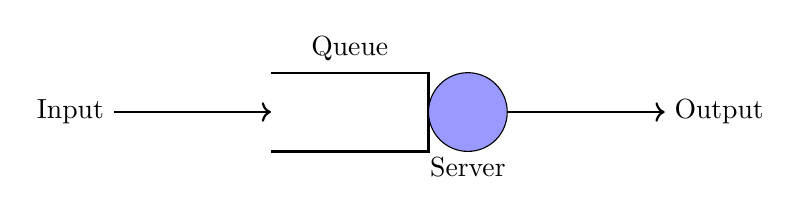
\begin{tikzpicture}
    % Draw the queue block (left-open rectangle)
    \draw[thick] (0, 0.5) -- (2, 0.5) -- (2, -0.5) -- (0, -0.5);
    \node at (1, 0.8) {Queue};

    % Draw the input arrow
    \draw[->, thick] (-2, 0) -- (0, 0);
    \node[left] at (-2, 0) {Input};

    % Draw the server (circle)
    \filldraw[fill=blue!40, draw=black] (2.5, 0) circle (0.5);
    \node at (2.5, -0.7) {Server};

    % Draw the output arrow
    \draw[->, thick] (3, 0) -- (5, 0);
    \node[right] at (5, 0) {Output};
\end{tikzpicture}
        \label{fig:simpleQblk}
        \caption{Block diagram of a simple, 1-D queue with one server and infinite capacity.}
    \end{figure}

\subsection{Terminology}
The above block diagram has a few terms used in it. A queue is formed by entities. What these entities are depends on the context provided by the application of the theory. For example, it could be jobs waiting to be executed at a server in a data center, or it could be humans waiting at a bank, or it could even be calls lined up at a call center. To address the requirements of the entity, the requirements again depend on the situation, there is an object we call a server. This server might be the processor, or the bank manager or the router.

Whenever a new entity is added to the queue, we call it as an arrival event. When the server addresses an entity, we call the event a departure event. In these notes we will refer to the entities in the queues as either arrivals or customers.

The state of the queue at any time instant is given by the number of customers at that time instant. Diagramatically, we will be using a state diagram quite frequently and hope that the reader is comfortable with it. If not, it is recommended that you refer \cite{pishro2014introduction}. 

\subsection{Kendall Notation}
A queue is characterized by how entities arrive to it, how they depart from it, how many servers are present, and if existant, what is the maximum length of the queue limited to.

\emph{Kendall's Notation} provides a condensed way to denote a queue. The general form is given by 
\begin{subequations}
    \begin{align}
        \mX / \mY / x / y 
    \end{align}
    where, 
    \begin{align*}
        \mX &= \text{Describes arrival statistics.}\\
        \mY &= \text{Describes the departure statistics.} \\
        x &= \text{Number of Servers.}\\
        y &= \text{Maximum length of the queue.} 
    \end{align*}
\end{subequations}
A frequently used statistics is \emph{Markovian}, where the process(es) of arrival and/or departure are Markov. `M' is used to abbreviate a Markovian statistics, `D' to denote Deterministic Timing, `G' for general statistics and `Geom' for Geometric. 

\subsection{Assumptions}

For our purposes of analysis, we make the following assumptions:
\begin{enumerate}
    \item If the server is not serving a customer i.e., it is free, then the arriving (next in line) customer is immediately assigned that server.
    \item Unless mentioned otherwise, if a server is busy, any new arrival joins the queue and waits for its chance.
    \item The time between the departure of a serviced customer and the start of the next customer is zero.
\end{enumerate}
Also, for simplicity, we will be sticking to a first-order analysis, thus, trading modeling accuracy for tractability and thereby insights.

\section{Service Discipline}
One thing we haven't addressed is the order in which the customers in a queue are called for service. One obvious rule is \emph{First Come First Serve} (FCFS) also known as \emph{First-In-First-Out} (FIFO). However, there arise scenarios where different disciplines are implemented. For example,  in case of mobile communication networks, emergency notifications regarding disasters must be prioritized over all other messages. Thus, in this case, the system might follow \emph{Last-In-First-Out-Pre-Emptive-Resume} (LIFOPR). For those working with embedded systems or computer architecture may be familiar with `memory stack' which is used to manage interrupts. In this case, the order in which different routines are serviced depends on the priorities of the interrupts in addition to the order in which they are triggered. For our purposes, we keep it simple and limit to FIFO service discipline.     

\chapter{M/M/1 Queue}
In this chapter, we will study the simplest kind of queue, the $M/M/1$ or also known as \emph{Markovian} queue. While the queue, once we get to its details may not seem realistic, it does provide valuable insights due to its mathematical tractability.

\dfn{M/M/1 (or Markovian) Queue}{
    A $M/M/1$ queue, also known as \emph{Markovian} queue is characterized as follows:
    \begin{enumerate}
        \item The arrival process is a Poisson Random process.
        \item There is a single server with the serving times being exponentially distributed. 
        \item There is no limit on the size of the queue. Also, the state of the queue is given by the number of arrivals/ customers in the queue at a given moment.
    \end{enumerate}  
}

Let's understand this queue slowly, one thing at a time.

\section{Arrivals}
By definition, the arrivals in an $M/M/1$ queue are a Poisson random process. If you are not familiar, its okay, since we will derive the entire framework from basic probability and a little bit of imagination.

Consider an experiment. You are watching a queue and tracking its movement. For ease, you divide the time axis into smaller intervals of length $\delta t$ such that there can atmost be a single arrival or no arrival. What decides whether there is a arrival or not? You toss a magical coin that is weirdly biased. If a toss results in heads, there is an arrival at the queue, else there is no arrival. The bias of the coin to land on its heads is proportional to the time interval i.e., $\delta t$. Thus, $\sP$(Heads) $ = \lambda \times \delta t$. 
If we consider an interval of length $T$, the number of slots $n \approx T / \delta t $. The experiment then reduces to $n$ coin flips with a coin with bias $\lambda \delta t$. 

The state of the system is given by the number of customers in the queue, $N(t)$ at some time instant $t$. From the coin analogy, we see that $N(t) \sim \text{Binomial}(n, p=\lambda\delta t)$
\begin{align}
    P_{N(t)}(k) &= \sP(N(t) = k) = \sP(\text{k arrivals in the interval [0, t]}) \\
    &= {n \choose k} (\lambda \delta t)^{k} (1 - \lambda \delta t)^{n-k} 
\end{align} 
Taking limit as $\delta t   \rightarrow 0$ and $\delta t \approx t / n$
\begin{align}
    \lim_{\delta t \rightarrow 0} P_{N(t)}(k) &= \lim_{\delta t \rightarrow 0}\frac{n!}{k! (n-k)!} \frac{\lambda^{k} t^{k}}{n^k} (1 - \frac{\lambda t}{n})^{n-k} \\
    &= \lim_{n \rightarrow \infty}\frac{n\times n-1 \times n-2 \times \dots \times n-(k-1)}{k!} \frac{\lambda^{k} t^{k}}{n^k} (1 - \frac{\lambda t}{n})^{n-k}\\
    &= \frac{1}{k!}\lim_{n \rightarrow \infty}(n/n\times (n-1)/n \times (n-2)/n \times \dots \times (n-(k-1))/n){\lambda^{k} t^{k}} (1 - \frac{\lambda t}{n})^{n-k}\\
    &= \frac{1}{k!}\lim_{n \rightarrow \infty}(1\times (1-1/n) \times (1-2/n) \times \dots \times (1-(k-1)/n)) \times{\lambda^{k} t^{k}} (1 - \frac{\lambda t}{n})^{n-k}\\
    &= \frac{\lambda^{k} t^{k}}{k!}\lim_{n \rightarrow \infty} (1 - \frac{\lambda t}{n})^{n-k}\\ 
    &= \frac{\lambda^{k} t^{k}}{k!}\lim_{n \rightarrow \infty} (1 - \frac{\lambda t}{n})^{n} \\
    &= \frac{\lambda^{k} t^{k}}{k!} e^{-\lambda t}
\end{align}
Thus, we get the result, 
\begin{align}
    P_{N(t)}(k) \sim \text{Poisson}(\lambda t) 
\end{align}

Lets make a few observations.
\begin{subequations}
    \begin{align}
        P_{N(\delta t)}(0) &= e^{-\lambda \delta t} \\
        &= 1 - \lambda \delta t + (\lambda \delta t)^2 - \ldots &&\quad \ldots \text{Taylor series expansion of } e^x.\\
        &\approx 1 - \lambda \delta t &&\quad \ldots \text{Neglecting higher order terms}.\\
        \\
        P_{N(\delta t)}(1) &= \lambda \delta t e^{-\lambda \delta t} \\ 
        &= \lambda \delta t (1 - \lambda \delta t) \\
        &= \lambda \delta t \\
        \\
        P_{N(t)}(k \geq 1) &\approx 0
    \end{align}    
    \label{eq:ApproxAssumptions}
\end{subequations}
Thus, we see that in the small interval $\delta t$, there is at most one arrival with probability of $\lambda \delta t$. Also there cannot be more than one arrival in the small interval.

\qs{What does the proportionality constant $\lambda$ signify?}{
    Consider the average number of arrivals per unit time i.e., 
    \begin{subequations}
        \begin{align}
            \bar{N} &= \frac{1}{t} \ExpVal[N(t)] \\
            \bar{N} &= \frac{1}{t} \sum_{k = 0}^{\infty} k P_{N(t)}(k) \\
            &= \frac{1}{t}\lambda t \\
            &= \lambda 
        \end{align}
    \end{subequations}
Hence, $\lambda$ is the rate of arrivals or mean arrivals per unit time. 
}
\nt{The Poisson random process has \emph{independent increments} and \emph{stationary increments}. }

Modeling a queue using such statistics has a fair share of advantages. Other than mathematically easy calculations, it is useful that splitting (thinning) and aggregation of Posson random processes results in other Poisson random processes.

\dfn{Splitting (Thinning) of Possion Process}{
Consider a parent Poisson Random process with rate $\lambda$. Then, if the arrivals in this processes ar e split into n different children with probabilities $p_1, p_2, \dots, p_n$, then the result is $n$ Poisson processes with rates $\lambda p_1, \lambda p_2, \dots, \lambda p_n$. Note that we must have $\sum p_i = 1$. See Fig.\ref{fig:split}.
}
\begin{figure}
    % First subfigure: Branching Diagram
    \begin{subfigure}[b]{0.45\textwidth}
        \centering
        
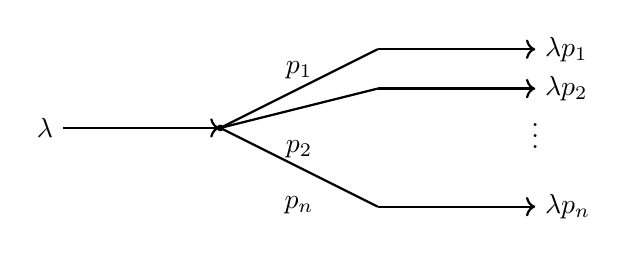
\begin{tikzpicture}
    % Draw the input arrow
    \draw[->, thick] (-2, 0) -- (-0.01, 0);
    \node[left] at (-2, 0) {$\lambda$};

    % Draw the branching point
    \filldraw (0, 0) circle (1pt);

    % Draw the branches
    \draw[thick] (0, 0) -- (2, 1);
    \draw[thick] (0, 0) -- (2, 0.5);
    \draw[thick] (0, 0) -- (2, -1);

    % Labels for probabilities
    \node[above] at (1, 0.5) {$p_1$};
    \node[above] at (1, -0.5) {$p_2$};
    \node[below] at (1, -0.75) {$p_n$};

    % Draw the output arrows for each branch
    \draw[->, thick] (2, 1) -- (4, 1);
    \draw[->, thick] (2, 0.5) -- (4, 0.5);
    \draw[->, thick] (2, -1) -- (4, -1);

    % Labels for the output flows
    \node[right] at (4, 1) {$\lambda p_1$};
    \node[right] at (4, 0.5) {$\lambda p_2$};
    \node at (4, 0) {$\vdots$};
    \node[right] at (4, -1) {$\lambda p_n$};
\end{tikzpicture}

        \caption{Splitting (Thinning of Poisson Process)}
        \label{fig:split}
    \end{subfigure}
    \hfill
    % Second subfigure: Merging Diagram
    \begin{subfigure}[b]{0.45\textwidth}
        \centering
        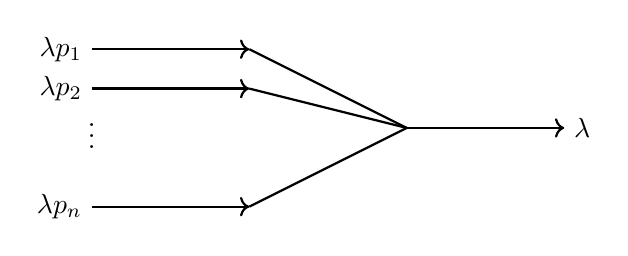
\begin{tikzpicture}
    % Draw the input arrows for each branch
    \draw[->, thick] (-4, 1.5) -- (-2, 1.5);
    \draw[->, thick] (-4, 1) -- (-2, 1);
    \draw[->, thick] (-4, -0.5) -- (-2, -0.5);

    % Labels for the input flows
    \node[left] at (-4, 1.5) {$\lambda p_1$};
    \node[left] at (-4, 1) {$\lambda p_2$};
    \node at (-4, 0.5) {$\vdots$};
    \node[left] at (-4, -0.5) {$\lambda p_n$};

    % Draw the merging point

    % Draw the branches
    \draw[thick] (-2, 1.5) -- (0, 0.5);
    \draw[thick] (-2, 1) -- (0, 0.5);
    \draw[thick] (-2, -0.5) -- (0, 0.5);

    % Draw the output arrow
    \draw[->, thick] (0, 0.5) -- (2, 0.5);
    \node[right] at (2, 0.5) {$\lambda$};
\end{tikzpicture}
        \caption{Merging of Poisson Process}
        \label{fig:merging}
    \end{subfigure}
    \label{fig:splitMerge}
\end{figure}

\dfn{Merging of Poisson Process}{
    Let $N_1(t)$ and $N_2(t)$ be two Poisson processes with rates $\lambda_1$ and $\lambda_2$ respectively. Then, the process $N(t)$ defined as $N(t) = N_1(t) + N_2(t)$ is also a Poisson random process with rate $\lambda_1 + \lambda_2$. See Fig.\ref{fig:merging}.
}

\subsection{State of the System - Alternative approach}
I would like to emphasize again that we are still considering only the arrivals and the state of the system is given by the number of customers in the system at a paticular time.

We can derive the distribution alternatively starting from Equations \ref{eq:ApproxAssumptions} as the basic setup or assumptions. 

\begin{figure}
    \centering
    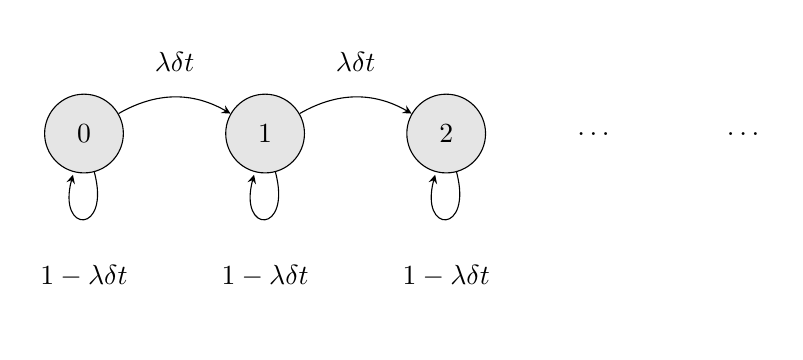
\begin{tikzpicture}[>=stealth, node distance=2.3cm, every node/.style={circle}]
    % Nodes
    \node (0) [draw, fill=gray!20, minimum size=10mm] {0};
    \node (1) [right of=0, draw, fill=gray!20, minimum size=10mm] {1};
    \node (2) [right of=1, draw, fill=gray!20, minimum size=10mm] {2};

    % Infinite continuation
    \node (ellipsis) [right of=2, xshift=1.5cm] {\dots};

    % Connecting nodes with edges and labels as plain text
    \path[->] (0) edge [bend left] node[above] {$\lambda \delta t$} (1)
              (1) edge [bend left] node[above] {$\lambda \delta t$} (2)
              ;

    % Self-loops with labels as plain text
    \path[->] (0) edge [loop below] node[below] {$1 - \lambda \delta t$} (0)
              (1) edge [loop below] node[below] {$1 - \lambda \delta t$} (1)
              (2) edge [loop below] node[below] {$1 - \lambda \delta t$} (2);

    % Ellipses for continuation
    \node at ($(2)!0.5!(ellipsis)$) {\dots};
\end{tikzpicture}

    \caption{State Transition Diagram for only arrivals}
    \label{fig:arrSTD}
\end{figure}

If $\sP(\text{Number of customers in the queue} = k, \text{at time}\ t) = P_{k}(t)$, then in a single $\delta t$ interval we can reach a state by either a single arrival or no arrival. We denote $p_{i,j}$ as the transition probability of going from state $i$ to $j$ in a $\delta t$ interval.
\begin{subequations}
    \begin{align}
        P_n(t+\delta t) &=  P_n(t)p_{n,n} + P_{n-1}(t)p_{n-1, n} \\
        &= P_n(t)(1 - \lambda \delta t) + P_{n-1}(t) (\lambda \delta t) &&\quad\ \ldots\ \text{See Fig.\ref{fig:arrSTD}} \\
        P_0(t + \delta t) &= P_0(t)p_{0, 0} \\
        &= P_0(t)(1 - \lambda \delta t)
    \end{align}
    \label{eq:altDer01}
\end{subequations}
Thus, we arrive at a recursive equation. However, we still need a starting (boundary) condition in order to get a solution. For this, note that to be at state 0, the system must have no arrival starting at state 0 (only arrivals remember?). Reorganizing Equations \ref{eq:altDer01},
\begin{subequations}
    \begin{align}
        \frac{P_n(t+\delta t) - P_n(t)}{\delta t} &= -\lambda P_n(t) + \lambda P_{n-1}(t) \\
        \frac{d P_n(t)}{dt} &= -\lambda P_n(t) + \lambda P_{n-1}(t) &&\quad\ \ldots\ \delta t \rightarrow 0.
    \end{align}
    Case $n = 0$ :
    \begin{align}
        \frac{d P_0(t)}{d t} = -\lambda P_0(t)
    \end{align} 
    Now those that are comfortable and in habit of working with differential equations may solve the above equation by visual inspection. Others may verify the solution by plugging the alleged function in the differential equation and verify that it satisfies the same. The solution is,
    \begin{align}
        P_0(t) = e^{-\lambda t}
    \end{align} 
    Similarly, 
    Case $n = 1$:
    \begin{align}
        \frac{d P_1(t)}{d t} &= \lambda P_1(t) + \lambda e ^{-\lambda t} \\
        P_1(t) &= \lambda t e^{-\lambda t}
    \end{align}
    Recognizing a pattern, we can generalize the result without explicit proof as,
    \begin{align}
        P_n(t) = \frac{(\lambda t)^n}{n!} e^{-\lambda t}
    \end{align}
\end{subequations}

\qs{\cite{RobertazziQ}}{If a telephone exchange is known to receive 100 calls a minute on average, what is the probability, that it gets 0 calls in 5 seconds.\\
\sol 0.00024.}

\subsection{Mean arrivals in an interval $[0, t]$}
\begin{subequations}
    \begin{align}
        \bar{N} &= \ExpVal[N(t)] \\
        &= \sum_{n=0}^{\infty} n P_n(t) \\
        &= \sum_{n=0}^{\infty} n \times \frac{(\lambda t)^n}{n!} e^{-\lambda t} \\
        &= e^{-\lambda t} (\lambda t) \sum_{n=1}^{\infty} \frac{(\lambda t)^{n-1}}{(n-1)!} \\
        &= e^{-\lambda t} (\lambda t) \sum_{n=0}^{\infty} \frac{(\lambda t)^n}{n!} \\
        &=  e^{-\lambda t} (\lambda t) e^{\lambda t} &&\quad\ \ldots\ \text{Taylor Series expansion of }e^x.\\
        \therefore \bar{N} &= \lambda t
    \end{align}
    \label{eq:Meanarr}
\end{subequations}

\nt{
- The results obtained is intuitively satisfactory since it states that on an average, the number of customers in a queue is proportional to the time interval of interest and the proportionality constant is given by the arrivals per unit time.

- This statistic can be used by a call center to determine a rough estimate of employees it may require to handle the calls.
}

\subsection{Variance of Number of arrivals in an interval $
[0, t]$}
Consider,
\begin{subequations}
    \begin{align}
        \ExpVal[N(t)^2] &= \sum_{n=0}^{\infty} n^2 \frac{(\lambda t)^n}{n!}e^{-\lambda t} \\
        &= \sum_{n=1}^{\infty} n^2 \frac{(\lambda t)^n}{n!}e^{-\lambda t} \\
        &= \sum_{n=1}^{\infty} n \frac{(\lambda t)^n}{(n-1)!}e^{-\lambda t} \\
        &= (\lambda t)e^{-\lambda t} \sum_{n=1}^{\infty}n \frac{(\lambda t)^{n-1}}{(n-1)!} \\
        &= (\lambda t)e^{-\lambda t} \sum_{n=0}^{\infty}(n+1) \frac{(\lambda t)^{n}}{(n)!} \\
        &= (\lambda t)e^{-\lambda t} \big[\sum_{n=0}^{\infty}n \frac{(\lambda t)^{n}}{(n)!}+ \sum_{n=0}^{\infty} \frac{(\lambda t)^{n}}{(n)!}\big] \\
        &= \lambda t e^{-\lambda t} [\lambda t e ^{\lambda t} + e^{\lambda t}] \\
        &= \lambda (1 + \lambda t) \\
        &= \lambda t + \lambda^2 t^2 \\
        \therefore var(N) &= \lambda t + \lambda^2 t^2 - (\lambda t)^2 \\
        &= \lambda t.
    \end{align}
    \label{eq:varArrivals}
\end{subequations}

\subsection{Inter-arrival times}
\dfn{Interarrival Time}{The time elasped between two consecutive arrival events is called the Interarrival time between those two events. Note that this quantity is a random quantity due to our setup.}
Let $T$ denote the interarrival time. Thus, 
\begin{subequations}
    \begin{align}
        F_P(t) = \sP(T < t) &= \sP(\text{Interarrival time is less than} t) \\
        &= 1 - \sP(\text{Interarrival time is more than} t) \\
        &= 1 - \sP(\text{No arrival in time interval of length} t) \\
        &= 1 - P_0(t) \\
        &= 1 - e^{-\lambda t}  
    \end{align}
    We recognize this CDF as that of an Exponentially distributed random variable. If not, we can get the PDF by differentiating as, 
    \begin{align}
        f_T(t) = \frac{d F_T(t)}{dt} = \lambda e^{-\lambda t}
    \end{align}
    Thus, the interarrival time $T$ is distributed as 
    \begin{align}
        T \sim \text{Exponential}(\lambda)
    \end{align}
    \label{eq:intertime}
\end{subequations}
Now's a good time to make some observations.
\nt{
    \begin{enumerate}
    \item The interarrival times are exponentially distributed meaning that the system memoryless. Intuitively, the current state of the system does not depend on the past. More concretely, say $\lambda = 10 $ min and we have had no arrival for 6 mins. Then the time after which we expect an arrival is still 10 mins and not 4 mins! Meaning it is as good as starting a new observation window. I recommend you to go through the proof of memorylessness property of Exponential distribution.
    \item Due to this, the state of the system at an instant is completely determined by the number of customers in the queue at that instant, there is no conditional dependence on the past.
    \item Discrete distribution with memoryless property is the Geometric distribution.  
\end{enumerate}
}
\qs{Where might we use this statistic?}{
    In a call center a worker could estimate the time between the calls he would receive. Then he can plan the next coffee break and how much he can converse with a colleague.
    
    More seriously, this statistic is important when it comes to scheduling other low priority tasks in a micro-processor or micro-controller based systems.
}

\section{Service}
We have ignored the poor server for a long time. Let's include him in our model now. In our $M/M/1$ model, we make the assumption that the service times for every customer are independent and identically distributed Exponential random variables with some rate $\mu$.

Thus, we make the following assumptions in addition to our previous ones.
\begin{subequations}
    \begin{align}
        \sP(\text{exactly 1 service in} [t, t+\delta t]) &= \mu \delta t \\
        \sP(\text{no service in} [t, t+\delta t]) &= 1 - \mu \delta t  \\
        \sP(\text{more than 1 service in} [t, t+\delta t]) &= 0.  
    \end{align}    
    \label{eq:assumDep}
\end{subequations}
Now the state of the system will be given by the number of customers in the queue as well as the one in service. 

The process resulting from such a system is called a \emph{birth-death} process in the literature.\cite{RobertazziQ, myReference}. The state transition diagram can be now updated to include the departures as well. See Fig.\ref{fig:mm1_std}. 
\begin{figure}
    \centering
    \begin{tikzpicture}[>=stealth, node distance=2.3cm,every node/.style={circle}]
    % Nodes
    \node (0) [draw, fill=gray!20, minimum size=10mm] {0};
    \node (1) [right of=0, draw, fill=gray!20, minimum size=10mm] {1};
    \node (2) [right of=1, draw, fill=gray!20, minimum size=10mm] {2};
    \node (3) [right of=2] {\dots};

    % Connecting nodes with edges and labels as plain text
    \path[->] (0) edge [bend left] node[above] {$\lambda$} (1) 
              (1) edge [bend left] node[above] {$\lambda $} (2)
              (2) edge [bend left] node[above] {$\lambda $} (3)
              ;

    \path[->] (1) edge [bend left] node[below] {$\mu$} (0)
    (2) edge [bend left] node[below] {$\mu$} (1)
    (3) edge [bend left] node[below] {$\mu$} (2)
    ;
    % Ellipses for continuation
    \node at ($(2)!0.5!(ellipsis)$) {\dots};
\end{tikzpicture}

    \caption{State Diagram for an $M/M/1$ system.}
    \label{fig:mm1_std}
\end{figure}

\subsection{State of the System}
Using the previous notation and differential equation approach, we now include the possiblity of a departure as well. Remember, we can jump only between adjacent states in $\delta t$. Also, we can either stay at zero to be in state 0 or depart from state 1.
\begin{subequations}
    \begin{align}
        P_n(t + \delta t) &= P_n(t) p_{n, n} + P_{n-1}(t)p_{n-1, n} + P_{n+1}(t) p_{n+1, n} \\
        P_0(t + \delta t) &= P_0(t)p_{0, 0} + P_1(t)p_{1, 0}
    \end{align}
    Now, 
    \begin{align}
        p_{n, n} &= \sP(\text{(No arrival and no departure) or (One arrival and One departure)}) \\ 
        &= (1 - \lambda \delta t)(1 - \mu \delta t) + (\lambda \delta t)(\mu \delta t) \\
        &\approx 1 - \lambda \delta t - \mu \delta t \\
        p_{n-1, n} &= \sP(\text{One arrival and no departure}) \\
        &= (\lambda \delta t)(1 - \mu \delta t) \\
        &\approx \lambda \delta t \\
        p_{n+1, n} &= \sP(\text{One departure and no arrival})\\
        &= (\mu \delta t)(1 - \lambda \delta t) \\
        & \approx \mu \delta t.  
    \end{align}  
    \label{eq:stateMM1}
\end{subequations}
\nt{Higher order terms have been neglected. Also, We cannot have a departure in state 0.}
Similar to previous derivations, we get the following equations:
\begin{subequations}
    \begin{align}
        \frac{d P_n(t)}{d t} &= -(\lambda + \mu) P_n(t) + \lambda P_{n-1}(t) + \mu P_{n+1}(t) \\
        \frac{d P_0(t)}{d t} &= -\lambda P_0(t) + \mu P_{}(t) 
    \end{align}
\end{subequations}
Solving these equations can be arduous. Thus, \cite{RobertazziQ} defines a new quantity. Let's see how this will come to our aid.
\dfn{Probability Flux}{
    Probability Flux is defined as the product of the probability of being in the state at which a transition originates and the transition rate to which the state travels next.
}
When the system is in equilibrium, we can say that the probability flux into a state equals the probability flux out of the state. This is called flow balancing and leads to what are known as local(global) balancing equations.

When in equilibrium we assume that $\frac{d P_n(t)}{t} = 0$
Thus, we get the following ``local balance equations'',
\begin{subequations}
    \begin{align}
        \lambda p_0 &= \mu p_1 &&\quad \implies p_1 = (\lambda / \mu) p_0 \\
        \lambda p_1 &= \mu p_2 &&\quad \implies p_2 = (\lambda / \mu) p_1 \\
        \vdots \\
        \lambda p_{n-1} &= \mu p_n &&\quad \implies p_{n-1} = (\lambda / \mu) p_n \\
        \vdots \\
    \end{align}
    Thus, we get the equation,
    \begin{align}
        p_n = (\lambda / \mu)^n p_0
    \end{align}
    \label{eq:lclBal}
\end{subequations}
Since the system must be in atleast one the possible states, the axioms of probability give us another equation, 
\begin{align}
    \sum_{i=0}^{num_{states}} p_i = 1.
\end{align}
Defining $\rho = \lambda / \mu$ for our $M/M/1$ with infinite states, we get,
\begin{align}
    p_0 + \rho p_0 + \rho^ 2 p_0 + \ldots &= 1 \\
    \therefore p_0 &= \frac{1}{\sum_{i=0}^{\infty} \rho^i}
\end{align}

Consider the case when $0 \leq \rho < 1$,
\begin{align}
    p_0 &= \frac{1}{\frac{1}{1 - \rho}} \\
    &= 1 - \rho.
\end{align}
\nt{Since $p_0$ is the probability that the queue is empty or unutilized, we call $\rho$ Utilization. When $\lambda$ is close to 0, we say we have very light load or zero load. Alternatively, if $\lambda \rightarrow \mu$, we say we have heavy load.}

\qs{Is it possible that $\rho > 1$?}{
    \sol{
        No. From the above derivation we see that the length of the queue will balloon up and blow up to be infinite in size. Hence, the system will not reach equilibrium, invalidating our above assumptions.
    }
}

\subsection{Average number of customers in $M/M/1$ queue}

We will now use the updated distribution.
\begin{subequations}
    \begin{align}
        \bar{N} = \ExpVal[N(t)] &= \sum_{n=0}^{\infty} n P_n(t) \\
        &= \sum_{n=0}^{\infty} n \rho^n p_0 \\
        &= (1 - \rho) \sum_{n=0}^{\infty} n \rho^n \\
        &= \rho (1 - \rho) \sum_{n=0}^{\infty} n \rho^{n-1}\\
        &= \rho (1 - \rho) \sum_{n=0}^{\infty} \frac{d \rho^n}{d \rho} \\
        &= \rho (1 - \rho) \frac{d\sum_{n=0}^{\infty}  \rho^n}{d \rho} \\
        &= \rho(1 - \rho) \frac{d 1/(1-\rho)}{d \rho} \\
        &= \frac{\rho}{1-\rho}
    \end{align}
    \label{eq:avgMM1}
\end{subequations}

\subsection{Variance of number of customers in $M/M/1$ queue}
Consider,
\begin{subequations}
    \begin{align}
        \ExpVal[N^2] &= \sum_{n=0}^{\infty} n^2 (1 - \rho)(\rho^n) \\
        &= (1 - \rho) \big[\sum_{n=0}^{\infty}n(n+1-1)\rho^n \big] \\
        &= (1 - \rho) \big[\sum_{n=0}^{\infty} n(n+1)\rho^n - \sum_{n=0}^{\infty}n\rho^n\big] \\
        &= (1 - \rho) \big[\rho^2 \sum_{n=0}^{\infty} n(n+1)\rho^{n-1} - \rho\sum_{n=0}^{\infty}n\rho^{n-1}\big] \\
        &= (1 - \rho) \big[\rho^2 \sum_{n=0}^{\infty} \frac{d^2\rho^{n+1}}{d\rho^2} - \rho\sum_{n=0}^{\infty}\frac{d\rho^{n}}{d \rho}\big] \\
        &= (1 - \rho) \big[\rho^2 \frac{d^2 \big(\sum_{n=1}^{\infty} \rho^n \big)}{d\rho^2} - \rho \frac{d \big(\sum_{n=0}^{\infty} \rho^n \big)}{d\rho}\big]
    \end{align}
    Using the formula for sum of Geometric Progression (for common ratio $< 1$),
    \begin{align}
        &= (1 - \rho) \big[ \rho^2 \frac{2}{(1-\rho)^3} + \frac{\rho}{(1 - \rho)^ 2}\big] \\
        &= \frac{\rho(1 + \rho)}{(1 - \rho)^ 2} \\
        \therefore \text{var}(N) &= \frac{\rho(1 + \rho)}{(1 - \rho)^ 2} - \frac{\rho^2}{(1 - \rho)^2} \\
        &= \frac{\rho}{(1 - \rho)^2}.
    \end{align} 
    \label{fig:varMM1}
\end{subequations}

\begin{figure}
    % First subfigure: Branching Diagram
    \begin{subfigure}[b]{0.55\textwidth}
        \centering
        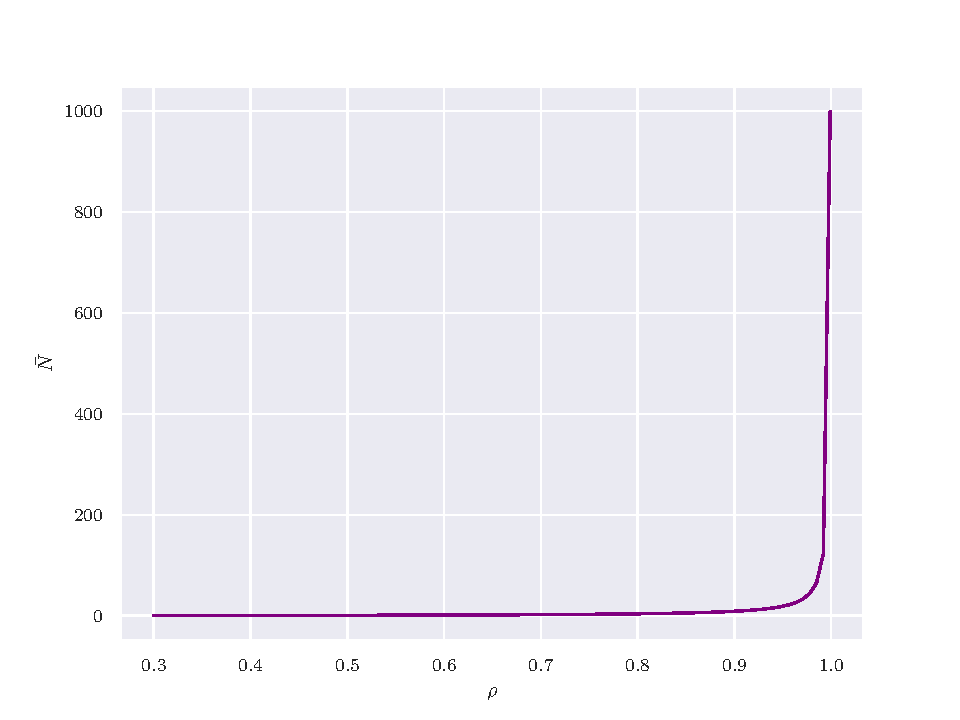
\includegraphics[width=\textwidth]{plots/avg_mm1.pdf}
        \caption{Average number of customers in an $M/M/1$ queue.}
        \label{fig:avgMM1_plot}
    \end{subfigure}
    \hfill
    % Second subfigure: Merging Diagram
    \begin{subfigure}[b]{0.55\textwidth}
        \centering
        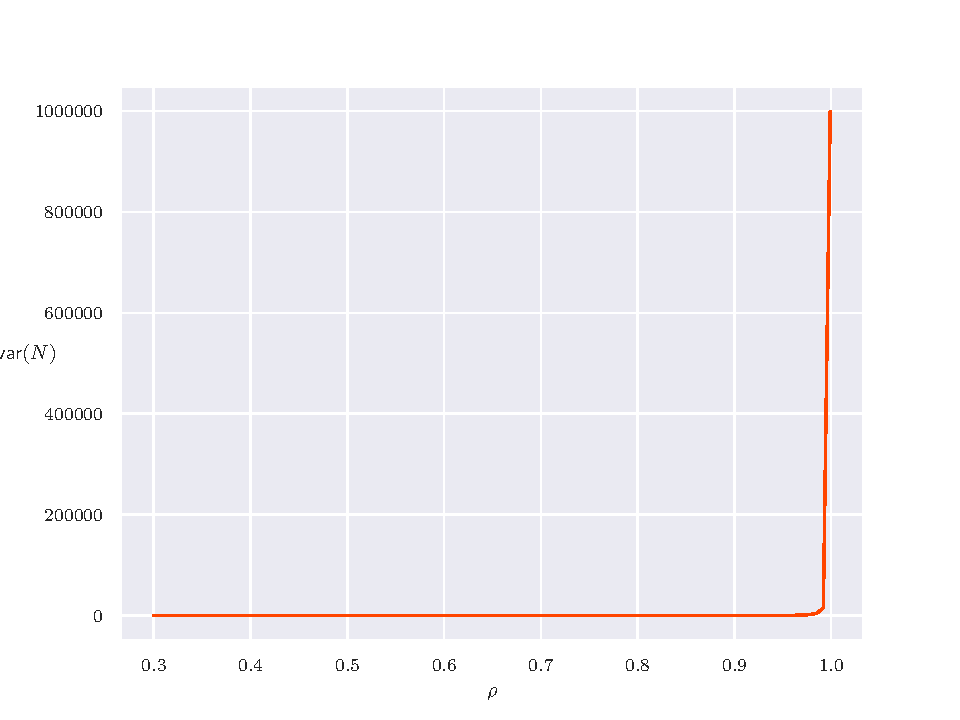
\includegraphics[width=\textwidth]{plots/var_mm1.pdf}
        \caption{Variance of number of customers in an $M/M/1$ queue.}
        \label{fig:varMM1_plot}
    \end{subfigure}
    \label{fig:mm1_stats}
\end{figure}

Please see Figs.\ref{fig:avgMM1_plot} and \ref{fig:varMM1_plot}. Note how the statistics blow up as the Utilization factor approaches 1.

\section{Little's Law}
Now that we have come up so far, lets try to relate the number in the queue with the time dimension.
\thm{Little's Law}{The mean number of customers in the queue, $\bar{N}$ is related to the rate of arrivals, $\lambda$, and the mean service time, $\bar{T}$ as 
\[
\bar{N} = \lambda \bar{T}.
\]
}  
\pf{Proof}{
    Consider a time interval of $[0, T]$.
    \begin{subequations}
        \begin{align}
            &\sP(\text{n customers in the queue after one departure})  \\ 
            &= \sP(\text{n customers arrive during the time spent in the queue by the depart customer.}) \\
            &= \int_{0}^{\infty}\sP(\text{n arrivals in during the interval} [0, T]\ |\ T=t) f_T(t) dt \\
            &= \int_{0}^{\infty}\sP(\text{n arrivals in during the interval} [0, t]) f_T(t) dt  \\
            &= \int_{0}^{\infty} \frac{(\lambda t)^n}{n!} e^{-\lambda} f_T(t) dt 
        \end{align}
        Now, using formula for expectation of a discrete random variable,
        \begin{align}
            \bar{N} &= \ExpVal[N] \\
            &= \sum_{n=0}^{\infty} nP_n(t) \\
            &= \sum_{n=0}^{\infty} n \int_{0}^{\infty} \frac{(\lambda t)^n}{n!} e^{-\lambda} f_T(t) dt \\
            &= \int_{0}^{\infty} \sum_{n=1}^{\infty} n \frac{(\lambda t)^n}{n!} e^{-\lambda t} f_T(t) dt \\
            &= \int_{0}^{\infty} \sum_{n=1}^{\infty} \lambda t \frac{(\lambda t)^{n-1}}{(n-1)!} e^{-\lambda t} f_T(t) dt \\
            &= \int_{0}^{\infty} \lambda t e^{-\lambda t} f_T(t) \sum_{n=0}^{\infty} \frac{(\lambda t)^n}{n!} dt \\
            &= \int_{0}^{\infty} \lambda t e^{-\lambda t} e^{\lambda t} f_T(t) dt &&\quad\ \ldots\ \text{Taylor series expansion of } e^x. \\ 
            &= \lambda \int_{0}^{\infty} t f_T(T) dt \\
            &= \lambda \ExpVal[T] \\
            &= \lambda \bar{T}.
        \end{align} 
        \label{eq:littleLaw}
    \end{subequations}
}
\nt{This result can be interpreted in simple way. The average waiting, $\bar{T}$, is the amount of time a customer is expected to wait once it arrives at the queue and until it leaves after being serviced. Moreover, $\lambda$ is the mean number of arrivals per unit time. Thus, in the time that a customer is in a queue, is likely to see $\lambda \bar{T}$ customers on an average.}

\chapter{Other Queues}

\section{Limitations of $M/M/1$ model}
While the previous queueing model was friendly enough that we could derive the nice results that we got, it isn't all that realistic. Recollect the assumptions that we made prior to embarking on the derivations. One of them was that the coin tosses that decide whether there is an arrival or not are independent and thus uncorrelated. However, how realistic is this assumption? 

Consider the case of a call center. In my experience at least, I have hardly ever got any resolution on my first call. What I mean is that once you make a call to a place, it is quite likely that you will call again. That means that the calls are not completely uncorrelated. However, this assumption is ok to make for a first-order analysis.

Next assumption that we made was that the queue could in theory grow limitlessly. This is quite impossible simply due to availability of limited resources and not to mention the patience one would require to stand in an infinite human queue. Hence, for next part of our analysis we consider a model with finite buffer length.

After this analysis, we ask why to limit our system to a single server queue? After all, the efficiency lies in parallelism. Thus, we consider the cases of `m' servers and a special case where $m = \infty$.

The analysis in the following sections will be similar to the previous ones and will heavily borrow from those sections. We request, that you are comfortable and up-to-speed on the concepts covered so far.

\section{$M/M/1/N$ - Finite Buffer Queue}

In this model, the queue size is limited to $N$. If there are $N$ customers in the queue, including one in the server, then any new arrivals are turnew away or dropped. To maintain the independence of arrivals, we further assume that the dropped customers do not arrive again. 

Due to the finite states we get a new state transition diagram shown in Fig.\ref{fig:mm1N_std}.
\begin{figure}
    \centering
    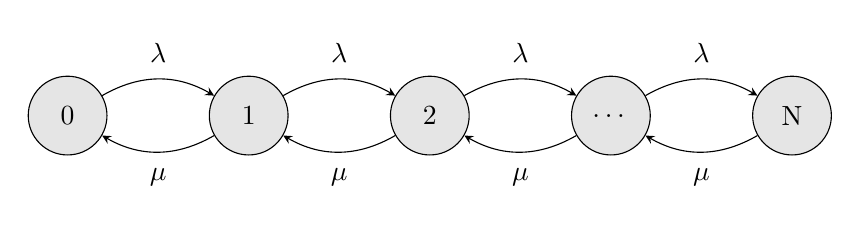
\begin{tikzpicture}[>=stealth, node distance=2.3cm,every node/.style={circle}]
    % Nodes without circles
    \node (0) [draw, fill=gray!20, minimum size=10mm] {0};
    \node (1) [right of=0, draw, fill=gray!20, minimum size=10mm] {1};
    \node (2) [right of=1, draw, fill=gray!20, minimum size=10mm] {2};
    \node (3) [right of=2, draw, fill=gray!20, minimum size=10mm] {$\dots$};
    \node (N) [right of=3, draw, fill=gray!20, minimum size=10mm] {N};

    % Edges with transition rates
    \draw[->, bend left] (0) to node[above] {$\lambda$} (1);
    \draw[->, bend left] (1) to node[above] {$\lambda$} (2);
    \draw[->, bend left] (2) to node[above] {$\lambda$} (3);
    \draw[->, bend left] (3) to node[above] {$\lambda$} (N);

    \draw[->, bend left] (1) to node[below] {$\mu$} (0);
    \draw[->, bend left] (2) to node[below] {$\mu$} (1);
    \draw[->, bend left] (3) to node[below] {$\mu$} (2);
    \draw[->, bend left] (N) to node[below] {$\mu$} (3);

\end{tikzpicture}
    \caption{State transition diagram for $M/M/1/N$ queue.}
    \label{fig:mm1N_std}
\end{figure}

Recollecting the local balance equations, we have under equilibrium,
\begin{subequations}
    \begin{align}
        p_n &= (\frac{\lambda}{\nu})^n p_0 =\rho^n p_0. 
    \end{align}
    Unlike previous model however, $0 \leq n \leq N$.
    Thus, to satisfy the axioms of probability, we must have,
    \begin{align}
        p_0 + p_1 + \dots + p_N &= 1 \\
        \implies p_0 + \rho p_0 + \rho^2 p_0 + \dots + \rho^N p_0 &= 1 \\
        p_0 (1 + \rho + \rho^2 + \dots + \rho ^N) &= 1 \\
        p_0 (\frac{1 - \rho ^ {N +1}}{1 - \rho}) &= 1 \\
        \therefore p_0 &= \frac{1 - \rho}{1 - \rho ^ {N + 1}} 
    \end{align} 
    Substituting in {3.1a}, for $0 \leq n \leq N$,
    \begin{align}
        p_n = \big(\frac{1 - \rho}{1 - \rho ^ {N + 1}}\big) \rho ^ n.
    \end{align}
    \label{eq:mm1n_eq}
\end{subequations}

\dfn{Blocking Probability}{
    The blocking probability is the probability that the queue buffer is full, i.e., $P_N(t)$. Using the derived equations, Blocking Probability is $\frac{(1-\rho)}{(1 - \rho^{N+1})} \rho^N$.
}
\nt{
    Using the blocking probability, we can find the mean number of customers turned away per unit time as $\lambda P_N(t)$.
}

\qs{What is $p_n$ when $\lambda / \mu = 1$?}{
    \sl{
        At $\lambda / \mu = 1$, $p_n$ assumes a $0/0$ form. We use L' Hopital's rule.
        \begin{align}
            \lim_{\rho \rightarrow 1} p_n &= lim_{\rho \rightarrow 1} \frac{1 - \rho}{1 - \rho^{N + 1}}\rho^n \\
            &= \lim_{\rho \rightarrow 1} \frac{-1}{-(N + 1)\rho^N}\\
            &= \frac{1}{N + 1}. 
        \end{align}
        }      
}

\nt{
    In this case, since the buffer size is limited, we can have $\lambda > \mu$ as the excess arrivals will simply be turned down or blocked. 
}

\begin{figure}
    % First subfigure: Branching Diagram
    \begin{subfigure}[b]{0.55\textwidth}
        \centering
        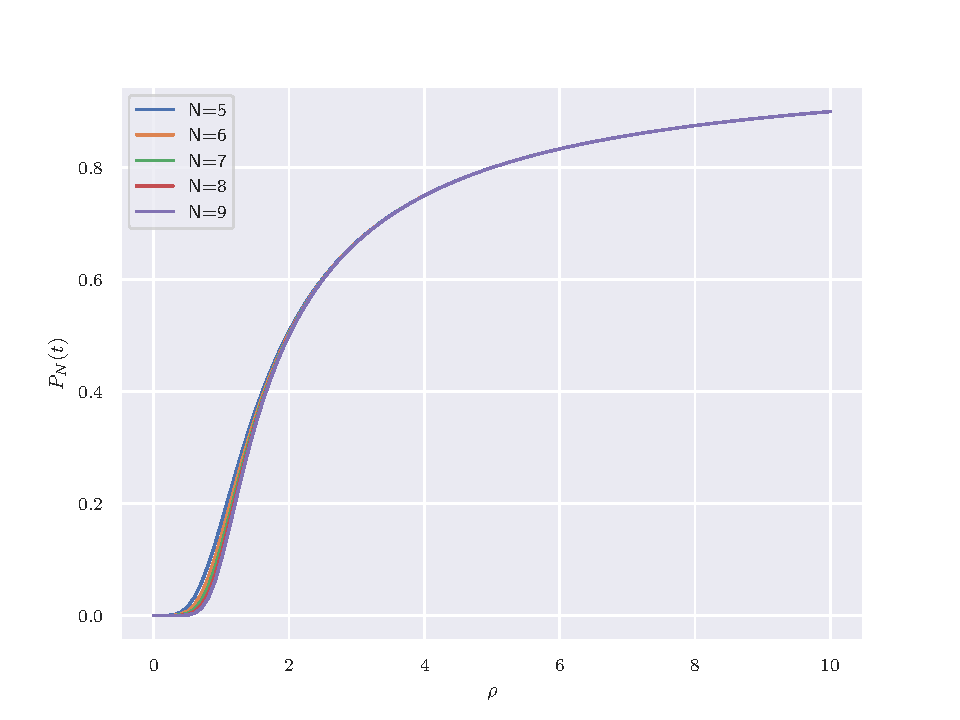
\includegraphics[width=\textwidth]{plots/blockProb_Nfix.pdf}
        \caption{Blocking probability as a function of $\rho$ ($N$ fixed).}
        \label{fig:blkprob_N}
    \end{subfigure}
    \hfill
    % Second subfigure: Merging Diagram
    \begin{subfigure}[b]{0.55\textwidth}
        \centering
        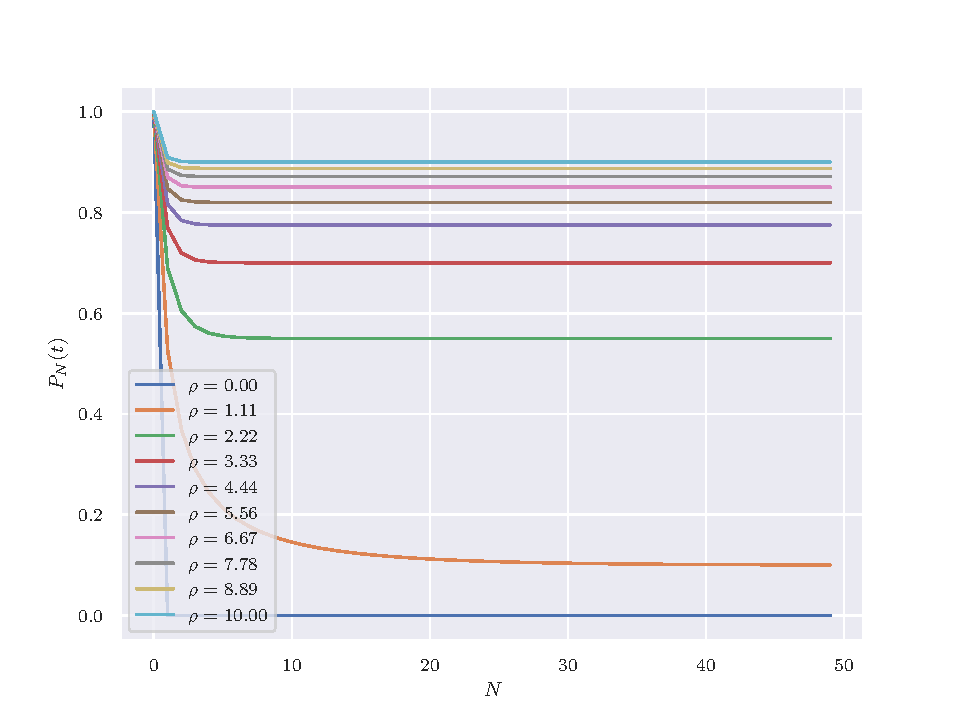
\includegraphics[width=\textwidth]{plots/blockProb_rhofix.pdf}
        \caption{Blocking probability as a function of $N$ ($\rho$ fixed).}
        \label{fig:blkprob_rho}
    \end{subfigure}
    \label{fig:blk_prob}
\end{figure}

We plot the blocking probabilities in Fig.\ref{fig:blkprob_N} and \ref{fig:blkprob_rho}. It concurs with our intuition that the blocking probability increases with increasing utilization ($\rho$) and decreases with increasing buffer length, $N$.

\section{$M/M/\infty$ - Infinite servers}

Now, we move on to the case of multiple server models. However, to warm, it is easier to consider the infinite server case as we will soon see. The setup we now have to work with is such that every arriving customer is assigned a personal server of rate $\mu$. Since, we have infinite servers, we don't mind it if the queue size increases limitlessly. 

\nt{
    If the system has $n$ customers at a time instant, as a whole the system has an aggregate output rate of $n\mu$. 
}
\begin{figure}[ht]   
    \begin{subfigure}[b]{0.55\textwidth}
        \centering
        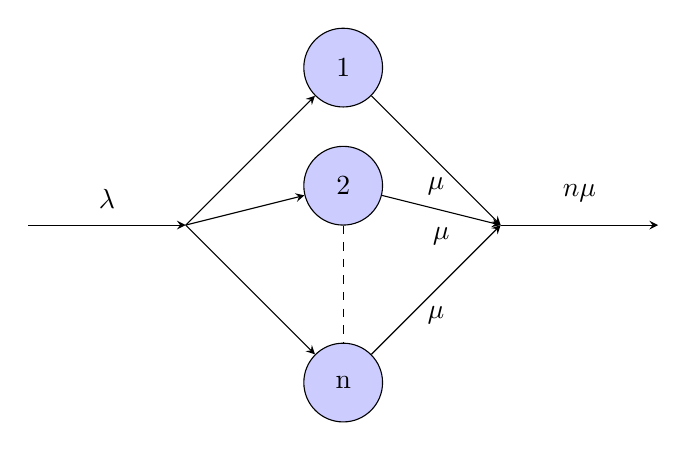
\begin{tikzpicture}[>=stealth, node distance=1.5cm, every node/.style={circle}]
    % Nodes
    \node (1) [{draw, fill=blue!20, minimum size=10mm, inner sep=0pt}]{1};
    \node (2) [{below of=1, draw, fill=blue!20, minimum size=10mm, inner sep=0pt}] {2};
    \node (n) [{below of=2, yshift=-1cm, draw, fill=blue!20, minimum size=10mm, inner sep=0pt}] {n};

    % Arrows for transitions
    \draw[->] (-2, -2) -- (1); 
    \draw[->] (-2, -2) -- (2); 
    \draw[->] (-2, -2) -- (n); 
    \draw[->] (1) -- (2, -2) node[midway, below] {$\mu$};
    \draw[->] (2) -- (2, -2) node[midway, below] {$\mu$};
    \draw[->] (n) -- (2, -2) node[midway, below] {$\mu$}; 

    % Connecting lines between nodes
    \draw[dashed] (2) -- (n);

    % Lambda arrow entering the chain
    \draw[->] (-4, -2) -- (-2, -2) node[midway, above] {$\lambda$};
    \draw[->] (2, -2) -- (4, -2) node[midway, above] {$n \mu$};
    
\end{tikzpicture}
        \caption{Flow diagram of an $M/M/\infty$ queue.}
        \label{fig:blk_mminfinite}
    \end{subfigure}
    \hfill
    \begin{subfigure}[b]{0.55\textwidth}
        \centering
        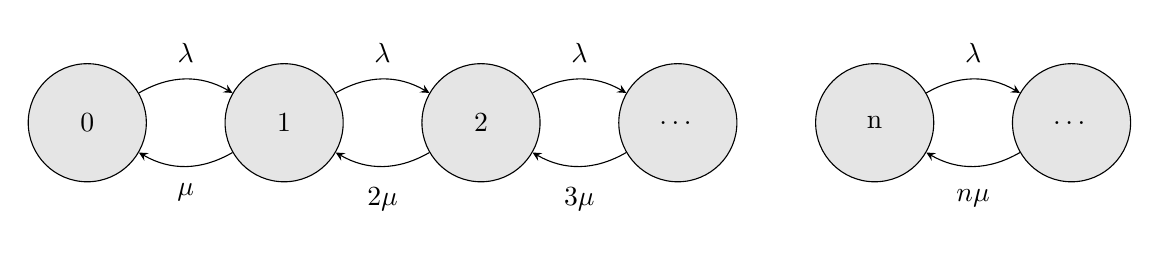
\begin{tikzpicture}[>=stealth, node distance=2.5cm, every node/.style={circle}]
    % Nodes
    \node (0) [{draw, fill=gray!20, minimum size=15mm, inner sep=0pt}] {0};
    \node (1) [{right of=0, draw, fill=gray!20, minimum size=15mm, inner sep=0pt}] {1};
    \node (2) [{right of=1, draw, fill=gray!20, minimum size=15mm, inner sep=0pt}] {2};
    \node (3) [{right of=2, draw, fill=gray!20, minimum size=15mm, inner sep=0pt}] {$\dots$};
    \node (n) [{right of=3, draw, fill=gray!20, minimum size=15mm, inner sep=0pt}] {n};
    \node (dots) [{right of=n, draw, fill=gray!20, minimum size=15mm, inner sep=0pt}] {$\dots$};

    % Transition arrows for arrivals
    \draw[->] (0) to[bend left] node[above] {$\lambda$} (1);
    \draw[->] (1) to[bend left] node[above] {$\lambda$} (2);
    \draw[->] (2) to[bend left] node[above] {$\lambda$} (3);
    \draw[->] (n) to[bend left] node[above] {$\lambda$} (dots);

    % Transition arrows for departures
    \draw[->] (1) to[bend left] node[below] {$\mu$} (0);
    \draw[->] (2) to[bend left] node[below] {$2\mu$} (1);
    \draw[->] (3) to[bend left] node[below] {$3\mu$} (2);
    \draw[->] (dots) to[bend left] node[below] {$n\mu$} (n);
\end{tikzpicture}

        \caption{State transition diagram of an $M/M/\infty$ queue.}
        \label{fig:std_mminfinite}
    \end{subfigure}
    \label{fig:mminfinite_dig}
\end{figure}
Using this setup, and refering to the state transition diagram shown in Fig.\ref{fig:std_mminfinite}, we get the below local balance equations.
\begin{subequations}
    \begin{align}
        \lambda p_0 &= \mu p_1  &&\implies p_1 = (\lambda / \mu) p_0 \\
        \lambda p_1 &= 2\mu p_2  &&\implies p_2 = (\lambda / 2\mu) p_1 \\
        \lambda p_2 &= 3\mu p_2  &&\implies p_3 = (\lambda / 3\mu) p_2 \\
    \end{align}
    Generalising, we get,
    \begin{align}
        p_n &= (\lambda / n \mu) p_{n-1} \\
        &= (\lambda / n \mu) (\lambda / (n - 1) \mu)  p_{n-2} \\
        \vdots \\
        &= \frac{\lambda ^ n}{n! \mu ^ n}p_0 
    \end{align}
    Since the probabilities must sum to 1, 
    \begin{align}
        p_0 + \frac{\lambda}{\mu} p_0 + \frac{\lambda^2}{2! \mu^2} p_0 + \frac{\lambda^3}{3!\mu^3} p_0 + \dots &= 1 \\
        \implies p_0(1 + \frac{\lambda}{\mu} +  \frac{\lambda^2}{2! \mu^2} + \frac{\lambda^3}{3!\mu^3} + \dots) &= 1 \\
        \implies p_0 (1 + \sum_{n=1}^{\infty} \frac{1}{n!}(\frac{\lambda}{\mu})^n) &= 1 \\
        \implies p_0 \times e^{\lambda / \mu} &= 1 &&\quad\ \ldots\ \text{Taylor series expansion of} e^x.
    \end{align}
    In summary, we thus have,
    \begin{align}
        p_0 &= e^{ - \lambda / \mu} \\
        p_n &= \frac{1}{n!}(\frac{\lambda}{\nu})^n e^{-\lambda / \mu} 
    \end{align}
    Defining $\rho = \lambda  / \mu$,
    \begin{align}
        p_n &= \frac{\rho^n}{n!} e^{-\rho}\\
        \therefore N &\sim \text{Poisson}(\rho)
    \end{align}
    \label{eq:mminfinite_eqs}
\end{subequations}

\section{$M/M/m$ - $m$ Parallel servers with a queue}

\begin{figure}[ht]   
        \centering
        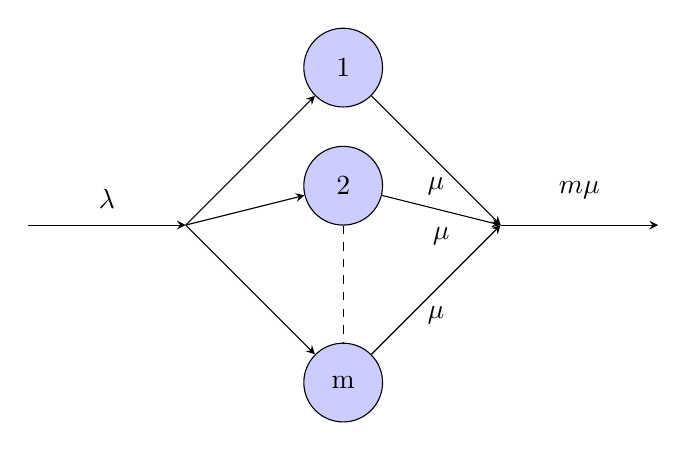
\begin{tikzpicture}[>=stealth, node distance=1.5cm, every node/.style={circle}]
    % Nodes
    \node (1) [{draw, fill=blue!20, minimum size=10mm, inner sep=0pt}]{1};
    \node (2) [{below of=1, draw, fill=blue!20, minimum size=10mm, inner sep=0pt}] {2};
    \node (m) [{below of=2, yshift=-1cm, draw, fill=blue!20, minimum size=10mm, inner sep=0pt}] {m};

    % Arrows for transitions
    \draw[->] (-2, -2) -- (1); 
    \draw[->] (-2, -2) -- (2); 
    \draw[->] (-2, -2) -- (m); 
    \draw[->] (1) -- (2, -2) node[midway, below] {$\mu$};
    \draw[->] (2) -- (2, -2) node[midway, below] {$\mu$};
    \draw[->] (m) -- (2, -2) node[midway, below] {$\mu$}; 

    % Connecting lines between nodes
    \draw[dashed] (2) -- (m);

    % Lambda arrow entering the chain
    \draw[->] (-4, -2) -- (-2, -2) node[midway, above] {$\lambda$};
    \draw[->] (2, -2) -- (4, -2) node[midway, above] {$m \mu$};
    
\end{tikzpicture}
        \caption{Flow diagram of an $M/M/m$ queue.}
    \label{fig:mmm_blk}
\end{figure}
\begin{figure}[ht]   
    \centering
    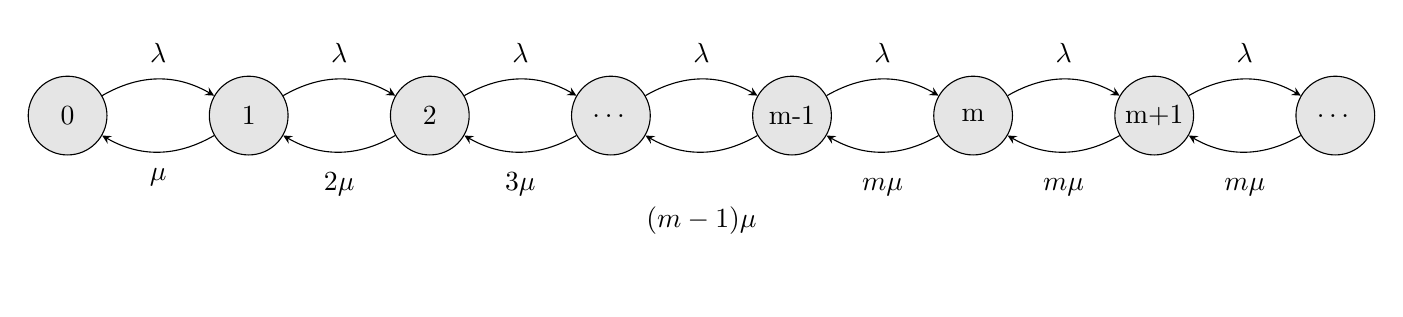
\begin{tikzpicture}[>=stealth, node distance=2.3cm, every node/.style={circle}]
    % Nodes
    \node (0) [{draw, fill=gray!20, minimum size=10mm, inner sep=0pt}] {0};
    \node (1) [{right of=0, draw, fill=gray!20, minimum size=10mm, inner sep=0pt}] {1};
    \node (2) [{right of=1, draw, fill=gray!20, minimum size=10mm, inner sep=0pt}] {2};
    \node (dots1) [{right of=2, draw, fill=gray!20, minimum size=10mm, inner sep=0pt}] {$\dots$};
    \node (m1) [{right of=dots1, draw, fill=gray!20, minimum size=10mm, inner sep=0pt}] {m-1};
    \node (m2) [{right of=m1, draw, fill=gray!20, minimum size=10mm, inner sep=0pt}] {m};
    \node (m3) [{right of=m2, draw, fill=gray!20, minimum size=10mm, inner sep=0pt}] {m+1};
    \node (dots2) [{right of=m3, draw, fill=gray!20, minimum size=10mm, inner sep=0pt}] {$\dots$};
  
  

    % Transition arrows for arrivals
    \draw[->] (0) to[bend left] node[above] {$\lambda$} (1);
    \draw[->] (1) to[bend left] node[above] {$\lambda$} (2);
    \draw[->] (2) to[bend left] node[above] {$\lambda$} (dots1);
    \draw[->] (dots1) to[bend left] node[above] {$\lambda$} (m1);
    \draw[->] (m1) to[bend left] node[above] {$\lambda$} (m2);
    \draw[->] (m2) to[bend left] node[above] {$\lambda$} (m3);
    \draw[->] (m3) to[bend left] node[above] {$\lambda$} (dots2);


    % Transition arrows for departures
    \draw[->] (1) to[bend left] node[below] {$\mu$} (0);
    \draw[->] (2) to[bend left] node[below] {$2\mu$} (1);
    \draw[->] (dots1) to[bend left] node[below] {$3\mu$} (2);
    \draw[->] (m1) to[bend left] node[below] {$(m-1)\mu$} (dots1);
    \draw[->] (m2) to[bend left] node[below] {$m \mu$} (m1);
    \draw[->] (m3) to[bend left] node[below] {$m \mu$} (m2);
    \draw[->] (dots2) to[bend left] node[below] {$m \mu$} (m3);

\end{tikzpicture}

    \caption{State transition diagram of an $M/M/m$ queue.}
\label{fig:mmm_std}
\end{figure}
Now we a realistic assumption and consider a model with only $m$ parallel servers. This results in a flow diagram, shown in Fig.\ref{fig:mmm_blk} and state transition diagram, shown in Fig.\ref{fig:mmm_std} . 
The transition rates are given in this case as,
\begin{align}
    \lambda(n) &= \lambda\ &&\quad\ , n=0, 1, 2, \ldots. \\
    \mu(n) &= n \mu\ &&\quad\ , n=1, 2,\ldots, m - 1. \\
    \mu(n) &= m \mu\ &&\quad\ , n=m, m+1, m+2,\ldots.   
\end{align}
Using these rates, we get the following balance equations,
\begin{subequations}
    \begin{align}
        p_1 &= (\lambda / \mu) p_0 \\
        p_2 &= (\lambda / 2 \mu) p_1 &&= (\lambda^2 / 2 \mu^2) p_0 \\
        p_3 &= (\lambda / 3 \mu) p_2 &&= (\lambda^3 / 3! \mu^3) p_0 \\
        \vdots \\
        p_m &= (\lambda / m \mu) p_{m-1} &&= (\lambda^m / m! \mu^m) p_0 \\
        p_{m+1} &= (\lambda / m \mu) p_m &&= (\lambda^{m+1} / m m! \mu^{m+1}) p_0 \\
        p_{m+2} &= (\lambda / m \mu) p_{m+1} &&= (\lambda^{m+2} / m^2 m! \mu^{m+2}) p_0 \\
        \vdots
    \end{align}
    \label{eq:mmm_eqs}    
    Generalising, we can write in short as,
    \begin{align}
        p_n &= \frac{\lambda^n}{n! \mu^n}\ &&\quad\ ,1 \leq n < m \\
        &= \frac{\lambda^n}{m^{n-m} m! \mu^n} p_0\ &&\quad\ ,n \geq m.  
    \end{align}
    Using the axioms of probability,
    \begin{align}
        \sum_{n=0}^{\infty} p_n &= 1\\
        \sum_{n=0}^{m-1} p_n + \sum_{n=m}^{\infty} p_n &= 1 \\ 
        p_0 \big(1 + \sum_{n=1}^{m-1} \frac{1}{n!} (\frac{\lambda}{\mu})^n + \sum_{n=m}^{\infty} \frac{1}{m^{n-m}} \frac{1}{m!} (\frac{\lambda}{\mu})^n
        \big) &= 1 \\
        \therefore p_0 &= \big[1 + \sum_{n=1}^{m-1} \frac{1}{n!} (\frac{\lambda}{\mu})^n + \sum_{n=m}^{\infty} \frac{1}{m^{n-m}} \frac{1}{m!} (\frac{\lambda}{\mu})^n
        \big] ^ {-1}. 
    \end{align}
\end{subequations}
Thus, we can find other state probabilities in equilibrium. One important probability that we can consider is the probability of the event that there will be a queue. There will be a queue whenever, all of the $m$ servers are busy and there are arrivals.
\qs{What is the queueing probability in an $M/M/m$ queue?}{
    \sol{
        \begin{align}
            \sP(\text{queueing}) &= \sP(n \geq m) \\
            &= \sum_{n=m}^{\infty} p_n \\
            &= \sum_{n=m}^{\infty} \frac{1}{m^{n-m}}\frac{1}{m!}(\frac{\lambda}{\mu})^n p_0 \\
            &= \frac{1}{m!}(\frac{\lambda}{\mu})^m \sum_{n=0}^{\infty}(\frac{\lambda}{m \mu})^n p_0\\
            &= \frac{1}{m!}(\frac{\lambda}{\mu})^m (\frac{1}{1 - \frac{\lambda}{m \mu}})p_0
         \end{align}
        Letting $\rho \coloneq \frac{\lambda}{m\mu}$,
        \begin{align}
            \sP(\text{queueing}) = \frac{1}{m!} (\frac{\lambda}{\mu})^m \frac{1}{1-\rho} p_0
        \end{align}
    }
}

\chapter{Appendix}
Only the bare minimum concepts have been covered here. I strongly advise that you go through the relevant material in \cite{pishro2014introduction}
\section{Random Processes}
\dfn{Random Process}{A random process is a collection (or a sequence) of variables usually indexed by time.
}
If the indexing variable is continuous, we refer to the process as a continuous-time random process and if the indexing variable is discrete, we call the process a discrete-time process. Thus, sampling a random process at a time instant gives a random variable. If this random variable is discrete, we call the process a discrete-valued process. Similarly, we define continuous-valued process. 

% References :
\bibliography{references}
\bibliographystyle{plain}

\end{document}
% \dfn{Limit of Sequence in }{Let be a sequence in}

% \qs{}{Is the set a closed set}
% \sol We have to take its complement and check whether that set is a open set i.e. if it is a union of open balls
% \nt{We will do topology in Normed Linear Space  (Mainly  and occasionally)using the language of Metric Space}
% \clm{Topology}{}{Topology is cool}
% \ex{Open Set and Close Set}{}